% Options for packages loaded elsewhere
\PassOptionsToPackage{unicode}{hyperref}
\PassOptionsToPackage{hyphens}{url}
\PassOptionsToPackage{dvipsnames,svgnames,x11names}{xcolor}
%
\documentclass[
  letterpaper,
  DIV=11,
  numbers=noendperiod]{scrreprt}

\usepackage{amsmath,amssymb}
\usepackage{lmodern}
\usepackage{iftex}
\ifPDFTeX
  \usepackage[T1]{fontenc}
  \usepackage[utf8]{inputenc}
  \usepackage{textcomp} % provide euro and other symbols
\else % if luatex or xetex
  \usepackage{unicode-math}
  \defaultfontfeatures{Scale=MatchLowercase}
  \defaultfontfeatures[\rmfamily]{Ligatures=TeX,Scale=1}
\fi
% Use upquote if available, for straight quotes in verbatim environments
\IfFileExists{upquote.sty}{\usepackage{upquote}}{}
\IfFileExists{microtype.sty}{% use microtype if available
  \usepackage[]{microtype}
  \UseMicrotypeSet[protrusion]{basicmath} % disable protrusion for tt fonts
}{}
\makeatletter
\@ifundefined{KOMAClassName}{% if non-KOMA class
  \IfFileExists{parskip.sty}{%
    \usepackage{parskip}
  }{% else
    \setlength{\parindent}{0pt}
    \setlength{\parskip}{6pt plus 2pt minus 1pt}}
}{% if KOMA class
  \KOMAoptions{parskip=half}}
\makeatother
\usepackage{xcolor}
\setlength{\emergencystretch}{3em} % prevent overfull lines
\setcounter{secnumdepth}{5}
% Make \paragraph and \subparagraph free-standing
\ifx\paragraph\undefined\else
  \let\oldparagraph\paragraph
  \renewcommand{\paragraph}[1]{\oldparagraph{#1}\mbox{}}
\fi
\ifx\subparagraph\undefined\else
  \let\oldsubparagraph\subparagraph
  \renewcommand{\subparagraph}[1]{\oldsubparagraph{#1}\mbox{}}
\fi

\usepackage{color}
\usepackage{fancyvrb}
\newcommand{\VerbBar}{|}
\newcommand{\VERB}{\Verb[commandchars=\\\{\}]}
\DefineVerbatimEnvironment{Highlighting}{Verbatim}{commandchars=\\\{\}}
% Add ',fontsize=\small' for more characters per line
\usepackage{framed}
\definecolor{shadecolor}{RGB}{241,243,245}
\newenvironment{Shaded}{\begin{snugshade}}{\end{snugshade}}
\newcommand{\AlertTok}[1]{\textcolor[rgb]{0.68,0.00,0.00}{#1}}
\newcommand{\AnnotationTok}[1]{\textcolor[rgb]{0.37,0.37,0.37}{#1}}
\newcommand{\AttributeTok}[1]{\textcolor[rgb]{0.40,0.45,0.13}{#1}}
\newcommand{\BaseNTok}[1]{\textcolor[rgb]{0.68,0.00,0.00}{#1}}
\newcommand{\BuiltInTok}[1]{\textcolor[rgb]{0.00,0.23,0.31}{#1}}
\newcommand{\CharTok}[1]{\textcolor[rgb]{0.13,0.47,0.30}{#1}}
\newcommand{\CommentTok}[1]{\textcolor[rgb]{0.37,0.37,0.37}{#1}}
\newcommand{\CommentVarTok}[1]{\textcolor[rgb]{0.37,0.37,0.37}{\textit{#1}}}
\newcommand{\ConstantTok}[1]{\textcolor[rgb]{0.56,0.35,0.01}{#1}}
\newcommand{\ControlFlowTok}[1]{\textcolor[rgb]{0.00,0.23,0.31}{#1}}
\newcommand{\DataTypeTok}[1]{\textcolor[rgb]{0.68,0.00,0.00}{#1}}
\newcommand{\DecValTok}[1]{\textcolor[rgb]{0.68,0.00,0.00}{#1}}
\newcommand{\DocumentationTok}[1]{\textcolor[rgb]{0.37,0.37,0.37}{\textit{#1}}}
\newcommand{\ErrorTok}[1]{\textcolor[rgb]{0.68,0.00,0.00}{#1}}
\newcommand{\ExtensionTok}[1]{\textcolor[rgb]{0.00,0.23,0.31}{#1}}
\newcommand{\FloatTok}[1]{\textcolor[rgb]{0.68,0.00,0.00}{#1}}
\newcommand{\FunctionTok}[1]{\textcolor[rgb]{0.28,0.35,0.67}{#1}}
\newcommand{\ImportTok}[1]{\textcolor[rgb]{0.00,0.46,0.62}{#1}}
\newcommand{\InformationTok}[1]{\textcolor[rgb]{0.37,0.37,0.37}{#1}}
\newcommand{\KeywordTok}[1]{\textcolor[rgb]{0.00,0.23,0.31}{#1}}
\newcommand{\NormalTok}[1]{\textcolor[rgb]{0.00,0.23,0.31}{#1}}
\newcommand{\OperatorTok}[1]{\textcolor[rgb]{0.37,0.37,0.37}{#1}}
\newcommand{\OtherTok}[1]{\textcolor[rgb]{0.00,0.23,0.31}{#1}}
\newcommand{\PreprocessorTok}[1]{\textcolor[rgb]{0.68,0.00,0.00}{#1}}
\newcommand{\RegionMarkerTok}[1]{\textcolor[rgb]{0.00,0.23,0.31}{#1}}
\newcommand{\SpecialCharTok}[1]{\textcolor[rgb]{0.37,0.37,0.37}{#1}}
\newcommand{\SpecialStringTok}[1]{\textcolor[rgb]{0.13,0.47,0.30}{#1}}
\newcommand{\StringTok}[1]{\textcolor[rgb]{0.13,0.47,0.30}{#1}}
\newcommand{\VariableTok}[1]{\textcolor[rgb]{0.07,0.07,0.07}{#1}}
\newcommand{\VerbatimStringTok}[1]{\textcolor[rgb]{0.13,0.47,0.30}{#1}}
\newcommand{\WarningTok}[1]{\textcolor[rgb]{0.37,0.37,0.37}{\textit{#1}}}

\providecommand{\tightlist}{%
  \setlength{\itemsep}{0pt}\setlength{\parskip}{0pt}}\usepackage{longtable,booktabs,array}
\usepackage{calc} % for calculating minipage widths
% Correct order of tables after \paragraph or \subparagraph
\usepackage{etoolbox}
\makeatletter
\patchcmd\longtable{\par}{\if@noskipsec\mbox{}\fi\par}{}{}
\makeatother
% Allow footnotes in longtable head/foot
\IfFileExists{footnotehyper.sty}{\usepackage{footnotehyper}}{\usepackage{footnote}}
\makesavenoteenv{longtable}
\usepackage{graphicx}
\makeatletter
\def\maxwidth{\ifdim\Gin@nat@width>\linewidth\linewidth\else\Gin@nat@width\fi}
\def\maxheight{\ifdim\Gin@nat@height>\textheight\textheight\else\Gin@nat@height\fi}
\makeatother
% Scale images if necessary, so that they will not overflow the page
% margins by default, and it is still possible to overwrite the defaults
% using explicit options in \includegraphics[width, height, ...]{}
\setkeys{Gin}{width=\maxwidth,height=\maxheight,keepaspectratio}
% Set default figure placement to htbp
\makeatletter
\def\fps@figure{htbp}
\makeatother
\newlength{\cslhangindent}
\setlength{\cslhangindent}{1.5em}
\newlength{\csllabelwidth}
\setlength{\csllabelwidth}{3em}
\newlength{\cslentryspacingunit} % times entry-spacing
\setlength{\cslentryspacingunit}{\parskip}
\newenvironment{CSLReferences}[2] % #1 hanging-ident, #2 entry spacing
 {% don't indent paragraphs
  \setlength{\parindent}{0pt}
  % turn on hanging indent if param 1 is 1
  \ifodd #1
  \let\oldpar\par
  \def\par{\hangindent=\cslhangindent\oldpar}
  \fi
  % set entry spacing
  \setlength{\parskip}{#2\cslentryspacingunit}
 }%
 {}
\usepackage{calc}
\newcommand{\CSLBlock}[1]{#1\hfill\break}
\newcommand{\CSLLeftMargin}[1]{\parbox[t]{\csllabelwidth}{#1}}
\newcommand{\CSLRightInline}[1]{\parbox[t]{\linewidth - \csllabelwidth}{#1}\break}
\newcommand{\CSLIndent}[1]{\hspace{\cslhangindent}#1}

\newcommand{\bs}{\symbf}
\newcommand{\mb}{\symbf}
\newcommand{\E}{\mathbb{E}}
\newcommand{\V}{\mathbb{V}}
\newcommand{\var}{\text{var}}
\newcommand{\cov}{\text{cov}}
\newcommand{\N}{\mathcal{N}}
\newcommand{\Bern}{\text{Bern}}
\newcommand{\Bin}{\text{Bin}}
\newcommand{\Pois}{\text{Pois}}
\newcommand{\Unif}{\text{Unif}}
\newcommand{\se}{\textsf{se}}
\newcommand{\au}{\underline{a}}
\newcommand{\du}{\underline{d}}
\newcommand{\Au}{\underline{A}}
\newcommand{\Du}{\underline{D}}
\newcommand{\xu}{\underline{x}}
\newcommand{\Xu}{\underline{X}}
\newcommand{\Yu}{\underline{Y}}
\renewcommand{\P}{\mathbb{P}}
\newcommand{\U}{\mb{U}}
\newcommand{\Xbar}{\overline{X}}
\newcommand{\Ybar}{\overline{Y}}
\newcommand{\real}{\mathbb{R}}
\newcommand{\bbL}{\mathbb{L}}
\renewcommand{\u}{\mb{u}}
\renewcommand{\v}{\mb{v}}
\newcommand{\M}{\mb{M}}
\newcommand{\X}{\mb{X}}
\newcommand{\Xmat}{\mathbb{X}}
\newcommand{\bfx}{\mb{x}}
\newcommand{\y}{\mb{y}}
\newcommand{\bfbeta}{\mb{\beta}}
\renewcommand{\b}{\symbf{\beta}}
\newcommand{\e}{\bs{\epsilon}}
\newcommand{\bhat}{\widehat{\mb{\beta}}}
\newcommand{\XX}{\Xmat'\Xmat}
\newcommand{\XXinv}{\left(\XX\right)^{-1}}
\newcommand{\hatsig}{\hat{\sigma}^2}
\newcommand{\red}[1]{\textcolor{red!60}{#1}}
\newcommand{\indianred}[1]{\textcolor{indianred}{#1}}
\newcommand{\blue}[1]{\textcolor{blue!60}{#1}}
\newcommand{\dblue}[1]{\textcolor{dodgerblue}{#1}}
\newcommand{\indep}{\perp\!\!\!\perp}
\newcommand{\inprob}{\overset{p}{\to}}
\newcommand{\indist}{\overset{d}{\to}}
\newcommand{\eframe}{\end{frame}}
\newcommand{\bframe}{\begin{frame}}
\newcommand{\R}{\textsf{\textbf{R}}}
\newcommand{\Rst}{\textsf{\textbf{RStudio}}}
\newcommand{\rfun}[1]{\texttt{\color{magenta}{#1}}}
\newcommand{\rpack}[1]{\textbf{#1}}
\newcommand{\rexpr}[1]{\texttt{\color{magenta}{#1}}}
\newcommand{\filename}[1]{\texttt{\color{blue}{#1}}}
\DeclareMathOperator*{\argmax}{arg\,max}
\DeclareMathOperator*{\argmin}{arg\,min}
\KOMAoption{captions}{tableheading}
\makeatletter
\@ifpackageloaded{tcolorbox}{}{\usepackage[many]{tcolorbox}}
\@ifpackageloaded{fontawesome5}{}{\usepackage{fontawesome5}}
\definecolor{quarto-callout-color}{HTML}{909090}
\definecolor{quarto-callout-note-color}{HTML}{0758E5}
\definecolor{quarto-callout-important-color}{HTML}{CC1914}
\definecolor{quarto-callout-warning-color}{HTML}{EB9113}
\definecolor{quarto-callout-tip-color}{HTML}{00A047}
\definecolor{quarto-callout-caution-color}{HTML}{FC5300}
\definecolor{quarto-callout-color-frame}{HTML}{acacac}
\definecolor{quarto-callout-note-color-frame}{HTML}{4582ec}
\definecolor{quarto-callout-important-color-frame}{HTML}{d9534f}
\definecolor{quarto-callout-warning-color-frame}{HTML}{f0ad4e}
\definecolor{quarto-callout-tip-color-frame}{HTML}{02b875}
\definecolor{quarto-callout-caution-color-frame}{HTML}{fd7e14}
\makeatother
\makeatletter
\makeatother
\makeatletter
\@ifpackageloaded{bookmark}{}{\usepackage{bookmark}}
\makeatother
\makeatletter
\@ifpackageloaded{caption}{}{\usepackage{caption}}
\AtBeginDocument{%
\ifdefined\contentsname
  \renewcommand*\contentsname{Table of contents}
\else
  \newcommand\contentsname{Table of contents}
\fi
\ifdefined\listfigurename
  \renewcommand*\listfigurename{List of Figures}
\else
  \newcommand\listfigurename{List of Figures}
\fi
\ifdefined\listtablename
  \renewcommand*\listtablename{List of Tables}
\else
  \newcommand\listtablename{List of Tables}
\fi
\ifdefined\figurename
  \renewcommand*\figurename{Figure}
\else
  \newcommand\figurename{Figure}
\fi
\ifdefined\tablename
  \renewcommand*\tablename{Table}
\else
  \newcommand\tablename{Table}
\fi
}
\@ifpackageloaded{float}{}{\usepackage{float}}
\floatstyle{ruled}
\@ifundefined{c@chapter}{\newfloat{codelisting}{h}{lop}}{\newfloat{codelisting}{h}{lop}[chapter]}
\floatname{codelisting}{Listing}
\newcommand*\listoflistings{\listof{codelisting}{List of Listings}}
\usepackage{amsthm}
\theoremstyle{definition}
\newtheorem{definition}{Definition}[chapter]
\theoremstyle{plain}
\newtheorem{theorem}{Theorem}[chapter]
\theoremstyle{definition}
\newtheorem{example}{Example}[chapter]
\theoremstyle{remark}
\renewcommand*{\proofname}{Proof}
\newtheorem*{remark}{Remark}
\newtheorem*{solution}{Solution}
\makeatother
\makeatletter
\@ifpackageloaded{caption}{}{\usepackage{caption}}
\@ifpackageloaded{subcaption}{}{\usepackage{subcaption}}
\makeatother
\makeatletter
\@ifpackageloaded{tcolorbox}{}{\usepackage[many]{tcolorbox}}
\makeatother
\makeatletter
\@ifundefined{shadecolor}{\definecolor{shadecolor}{rgb}{.97, .97, .97}}
\makeatother
\makeatletter
\makeatother
\ifLuaTeX
  \usepackage{selnolig}  % disable illegal ligatures
\fi
\IfFileExists{bookmark.sty}{\usepackage{bookmark}}{\usepackage{hyperref}}
\IfFileExists{xurl.sty}{\usepackage{xurl}}{} % add URL line breaks if available
\urlstyle{same} % disable monospaced font for URLs
\hypersetup{
  pdftitle={A User's Guide to Statistical Inference and Regression},
  pdfauthor={Matthew Blackwell},
  colorlinks=true,
  linkcolor={blue},
  filecolor={Maroon},
  citecolor={Blue},
  urlcolor={Blue},
  pdfcreator={LaTeX via pandoc}}

\title{A User's Guide to Statistical Inference and Regression}
\author{Matthew Blackwell}
\date{}

\begin{document}
\maketitle
\ifdefined\Shaded\renewenvironment{Shaded}{\begin{tcolorbox}[borderline west={3pt}{0pt}{shadecolor}, boxrule=0pt, interior hidden, breakable, frame hidden, enhanced, sharp corners]}{\end{tcolorbox}}\fi

\renewcommand*\contentsname{Table of contents}
{
\hypersetup{linkcolor=}
\setcounter{tocdepth}{2}
\tableofcontents
}
\bookmarksetup{startatroot}

\hypertarget{preface}{%
\chapter*{Preface}\label{preface}}
\addcontentsline{toc}{chapter}{Preface}

\markboth{Preface}{Preface}

\includegraphics{./assets/img/linear-approximation.png}

This is a set of notes for
\href{https://gov2002.mattblackwell.org}{Government 2002: Quantitative
Social Science Methods II} at Harvard University taught by
\href{https://www.mattblackwell.org}{Matthew Blackwell}. The goal of
this text is to provide a rigorous yet accessible introduction to the
foundational topics in statistical inference with a special application
to linear regression, a workhorse tool in the social sciences. The
material is intended for first-year PhD students in political science,
but it may be of interest more broadly. Much of the material has been
adopted from various sources (far too many to recount now), but this
book is especially indebted to the following texts:

\begin{itemize}
\tightlist
\item
  Hansen, Bruce.
  \href{https://www.amazon.com/Probability-Statistics-Economists-Bruce-Hansen/dp/0691235945/}{\emph{Probability
  \& Statistics for Economists}}. Princeton University Press.
\item
  Hansen, Bruce.
  \href{https://www.amazon.com/Econometrics-Bruce-Hansen/dp/0691235899/}{\emph{Econometrics}}.
  Princeton University Press.
\item
  Wasserman, Larry.
  \href{https://link.springer.com/book/10.1007/978-0-387-21736-9}{\emph{All
  of Statistics: A Concise Course in Statistical Inference}}. Springer.
\item
  Wooldridge, Jeffrey.
  \href{https://mitpress.mit.edu/9780262232586/econometric-analysis-of-cross-section-and-panel-data/}{\emph{Econometric
  Analysis of Cross Section and Panel Data}}
\end{itemize}

You can find the source for this book at
\url{https://github.com/mattblackwell/gov2002-book}. Any typos or errors
can be reported at
\url{https://github.com/mattblackwell/gov2002-book/issues}. Thanks for
reading.

This is a Quarto book. To learn more about Quarto books visit
\url{https://quarto.org/docs/books}.

\(\,\)

\bookmarksetup{startatroot}

\hypertarget{introduction}{%
\chapter{Introduction}\label{introduction}}

\(\,\)

This book, like so many books before it, will try to teach you
statistics. The field of statistics describes how we learn about the
world from quantitative data. In the social sciences, the vast majority
of empirical studies use statistical methods to provide evidence for
their arguments. While it is possible to conduct quantitative research
without understanding statistics, one must advise against it.
Quantitative research involves a host of \emph{choices} about what model
to use, what variables to include, what tuning parameters to set, what
assumptions to make, and so on. Without a deep understanding of
statistics, you will find these choices bewildering and often yield to
the default settings of your statistical software. The goal of this book
is to give you the foundation to confidently make those choices for your
specific application.

We will focus on two key goals in this book.

\begin{enumerate}
\def\labelenumi{\arabic{enumi}.}
\item
  \textbf{Understand the basic ways to assess estimators} With
  quantitative data, we often want to make statistical inferences about
  some unknown feature of the world. We use estimators (which are just
  ways of summarizing our data) to estimate these features. One major
  goal of this book is to show the basics of this task at a general
  enough level to be applicable to almost any estimator that you are
  likely to encounter in research. The ideas of bias, sampling variance,
  consistency, and asymptotic normality are common to such a large swath
  of (frequentist) inference that you get a tremendous return on your
  investment of time in these topics. Understand these core ideas and
  you will have a language to analyze any fancy new estimator that pops
  up in the next few decades.
\item
  \textbf{Apply these ideas to estimation of regressions} This book will
  apply these ideas to one particular workhorse task in the social
  sciences: estimating regression functions. So many methods are either
  use regression estimators like ordinary least squares or extend it in
  some way. Understanding how these estimators work is vital for
  conducting research in the social sciences. Regression and regression
  estimators also provide an entry point for discussing parametric
  models explicitly as approximation and projections rather than as
  rigid assumptions about the truth of a given specification.
\end{enumerate}

Why write a book on statistics and regression when so many already
exist? Aside from hubris, my goal in this book is to find a level of
mathematical sophistication that will challenge and push political
scientists to develop stronger foundations in the material. While some
textbooks at this level exist in statistics and economics, they tend to
focus on applications less relevant to political science. This book
attempts to correct this.

\bookmarksetup{startatroot}

\hypertarget{estimation}{%
\chapter{Estimation}\label{estimation}}

\hypertarget{introduction-1}{%
\section{Introduction}\label{introduction-1}}

When studying probability, we assumed that we knew the parameter of a
distribution (the mean or the variance) and used probability theory to
understand what kind of data we would observe. Estimation and inference
put this engine in reverse and try to learn some aspect of the
data-generating process using only our observed data. There are two main
goals here: \textbf{estimation}, which is how we formulate our best
guess about a parameter of the DGP, and \textbf{inference}, which is how
we formalize and express uncertainty about our estimates.

\includegraphics{./assets/img/two-direction.png}

\leavevmode\vadjust pre{\hypertarget{exm-rct}{}}%
\begin{example}[Randomized control trial]\label{exm-rct}

Suppose we are conducting a randomized experiment on framing effects.
All respondents receive some factual information about current levels of
immigration. The message for the treatment group (\(D_i = 1\)) has an
additional framing of the positive benefits of immigration, while the
control group (\(D_i = 0\)) receives no additional framing. The outcome
is a binary outcome on whether the respondent supports increasing legal
immigration limits (\(Y_i = 1\)) or not (\(Y_i = 0\)). The observed data
consists of \(n\) pairs of random variables, the outcome, and the
treatment assignment: \(\{(Y_1, D_1), \ldots, (Y_n, D_n)\}\). Define the
two sample means/proportions in each group as \[
\Ybar_1 = \frac{1}{n_1} \sum_{i: D_i = 1} Y_i,  \qquad\qquad \Ybar_0 = \frac{1}{n_0} \sum_{i: D_i = 0} Y_i,
\] where \(n_1 = \sum_{i=1}^n D_i\) is the number of treated units and
\(n_0 = n - n_1\) is the number of control units.

A standard estimator for the treatment effect in a study like this would
be the difference in means, \(\Ybar_1 - \Ybar_0\). But this is only one
possible estimator. We could also estimate the effect by taking this
difference in means separately by party identification and then
averaging those party-specific effects by the size of those groups. This
estimator is commonly called a \textbf{poststratification} estimator,
but it's unclear at first glance which of these two estimators we should
prefer.

\end{example}

What are the goals of studying estimators? In short, we prefer to use
\textbf{good} estimators rather than \textbf{bad} estimators. But what
makes an estimator good or bad? You probably have some intuitive sense
that, for example, an estimator that returns the value 3 is bad. Still,
it will be helpful for us to formally define and explore some properties
of estimators that will allow us to compare them and choose the good
over the bad.

\hypertarget{samples-and-populations}{%
\section{Samples and populations}\label{samples-and-populations}}

For most of this class, we'll focus on a relatively simple setting where
we have a set of random vectors \(\{X_1, \ldots, X_n\}\) that are
\textbf{independent and identically distributed} (iid) draws from a
distribution with cumulative distribution function (cdf) \(F\). They are
independent in that the random vectors \(X_i\) and \(X_j\) are
independent for all \(i \neq j\), and they are ``identically
distributed'' in the sense that each of the random variables \(X_i\)
have the same marginal distribution, \(F\).

You can think of each vector, \(X_i\), as the rows in your data frame.
Note that we're being purposely vague about this cdf---it simply
represents the unknown distribution of the data, otherwise known as the
\textbf{data generating process} (DGP). Sometimes \(F\) is also referred
to as the \textbf{population distribution} or even just
\textbf{population}, which has its roots in viewing the data as a random
sample from some larger population. As a shorthand, we often say that
the collection of random vectors \(\{X_1, \ldots, X_n\}\) is a
\textbf{random sample} from population \(F\) if \(\{X_1, \ldots, X_n\}\)
is iid with distribution \(F\). The \textbf{sample size} \(n\) is the
number of units in the sample.

Two metaphors can help build intuition about the concept of viewing the
data as an iid draw from \(F\):

\begin{enumerate}
\def\labelenumi{\arabic{enumi}.}
\tightlist
\item
  \textbf{Random sampling}. Suppose we have a population of size \(N\)
  that is much larger than our sample size \(n\), and we take a simple
  random sample of size \(n\) from this population. Then the
  distribution of the data in the random sample will be iid draws from
  the population distribution of the variables we are sampling. For
  instance, suppose we take a random sample from a population of US
  citizens where the population proportion of Democratic party
  identifiers is 0.33. Then if we randomly sample \(n = 100\) US
  citizens, each data point \(X_i\) will be distributed Bernoulli with
  probability of success 0.33.
\item
  \textbf{Groundhog Day}. Random sampling does not always make sense as
  a justification for iid data, especially when the units are not
  samples at all but rather countries, states, or subnational units. In
  this case, we have to appeal to a thought experiment where \(F\)
  represents the fundamental uncertainty in the data-generating process.
  The metaphor here is that if we could re-run history many times, like
  the 1993 American classic comedy \emph{Groundhog Day}, data and
  outcomes would change slightly due to the inherently stochastic nature
  of the world. The iid assumption, then, is that each of the units in
  our data has the same DGP producing this data or the same distribution
  of outcomes under the \emph{Groundhog Day} scenario.{[}1{]}
\end{enumerate}

Note that there are many situations where the iid assumption is not
appropriate. We will cover some of those later in the semester. But much
of the innovation and growth in statistics over the last 50 years has
been figuring out how to perform statistical inference when iid does not
hold. Often, the solutions are specific to the type of iid violation you
have (spatial, time-series, network, or clustered). As a rule of thumb,
though, if you suspect iid is incorrect, your uncertainty statements
will likely be overconfident (for example, confidence intervals, which
we'll cover later, are too small).

\hypertarget{point-estimation}{%
\section{Point estimation}\label{point-estimation}}

\hypertarget{quantities-of-interest}{%
\subsection{Quantities of interest}\label{quantities-of-interest}}

We aim to learn about the data-generating process, represented by the
cdf, \(F\). We might be interested in estimating the cdf at a general
level or only some feature of the distribution, like a mean or
conditional expectation function. We will almost always have a
particular quantity in mind, but we'll introduce estimation at a general
level. So we'll let \(\theta\) represent the quantity of interest.
\textbf{Point estimation} describes how we obtain a single ``best
guess'' about \(\theta\).

\begin{tcolorbox}[enhanced jigsaw, title=\textcolor{quarto-callout-note-color}{\faInfo}\hspace{0.5em}{Note}, breakable, titlerule=0mm, opacityback=0, rightrule=.15mm, bottomrule=.15mm, colframe=quarto-callout-note-color-frame, coltitle=black, colbacktitle=quarto-callout-note-color!10!white, bottomtitle=1mm, toptitle=1mm, colback=white, arc=.35mm, opacitybacktitle=0.6, toprule=.15mm, leftrule=.75mm, left=2mm]

Some refer to quantities of interest as \textbf{parameters} or
\textbf{estimands} (that is, the target of estimation).

\end{tcolorbox}

\leavevmode\vadjust pre{\hypertarget{exm-prop}{}}%
\begin{example}[Population mean]\label{exm-prop}

Suppose we wanted to know the proportion of US citizens who support
increasing legal immigration in the US, which we denote as \(Y_i = 1\).
Then our quantity of interest is the mean of this random variable,
\(\mu = \E[Y_i]\), which is the probability of randomly drawing someone
from the population supporting increased legal immigration.

\end{example}

\leavevmode\vadjust pre{\hypertarget{exm-var}{}}%
\begin{example}[Population variance]\label{exm-var}

Feeling thermometer scores are a prevalent way to assess how a survey
respondent feels about a particular person or group. A survey asks
respondents how warmly they feel about a group from 0 to 100, which we
will denote \(Y_i\). We might be interested in how polarized views are
on a group in the population, and one measure of polarization could be
the variance, or spread, of the distribution of \(Y_i\) around the mean.
In this case, \(\sigma^2 = \V[Y_i]\) would be our quantity of interest.

\end{example}

\leavevmode\vadjust pre{\hypertarget{exm-rct-ii}{}}%
\begin{example}[RCT continued]\label{exm-rct-ii}

In Example~\ref{exm-rct}, we discussed a typical estimator for an
experimental study with a binary treatment. The goal of that experiment
is to learn about the difference between two conditional probabilities
(or expectations): the average support for increasing legal immigration
in the treatment group, \(\mu_1 = \E[Y_i \mid D_i = 1]\), and the same
average in the control group, \(\mu_0 = \E[Y_i \mid D_i = 0]\). This
difference, \(\mu_1 - \mu_0\), is a function of unknown features of
these two conditional distributions.

\end{example}

Each of these is a function of the (possibly joint) distribution of the
data, \(F\). In each of these, we are not necessarily interested in the
entire distribution, just summaries of it (central tendency, spread). Of
course, there are situations where we are also interested in the
complete distribution.

\hypertarget{estimators}{%
\subsection{Estimators}\label{estimators}}

When our sample size is more than a few observations, it makes no sense
to work with the raw data, \(X_1, \ldots, X_n\), and we inevitably will
need to \emph{summarize} the data in some way. We can represent this
summary as a function, \(g(x_1, \ldots, x_n)\), which might be the
formula for the sample mean or sample variance. This function is just a
regular function that takes in \(n\) numbers (or vectors) and returns a
number (or vector). We can also define a random variable based on this
function, \(Y = g(X_1, \ldots, X_n)\), which inherits its randomness
from the randomness of the data. Before we see the data, we don't know
what values of \(X_1, \ldots, X_n\) we will see, so we don't know what
value of \(Y\) we'll see either. We call the random variable
\(Y = g(X_1, \ldots, X_n)\) a \textbf{statistic} (or sometimes sample
statistics), and we refer to the probability distribution of a statistic
\(Y\) as the \textbf{sampling distribution} of \(Y\).

\begin{tcolorbox}[enhanced jigsaw, title=\textcolor{quarto-callout-warning-color}{\faExclamationTriangle}\hspace{0.5em}{Warning}, breakable, titlerule=0mm, opacityback=0, rightrule=.15mm, bottomrule=.15mm, colframe=quarto-callout-warning-color-frame, coltitle=black, colbacktitle=quarto-callout-warning-color!10!white, bottomtitle=1mm, toptitle=1mm, colback=white, arc=.35mm, opacitybacktitle=0.6, toprule=.15mm, leftrule=.75mm, left=2mm]

There is one potential confusion in how we talk about ``statistics.''
Just above, we defined a statistic as a random variable based on it
being a function of random variables (the data). But we sometimes refer
to the calculated value as a statistic as well, which is a specific
number that you see in your R output. To be precise, we should call the
latter the \textbf{realized value} of the statistic, but message
discipline is difficult to enforce in this context. A simple example
might help. Suppose that \(X_1\) and \(X_2\) are the results of a roll
of two standard six-sided dice. Then the statistic \(Y = X_1 + X_2\) is
a random variable that has a distribution over the numbers from \{2,
\ldots, 12\} that describes our uncertainty over what the sum will be
\emph{before we roll the dice}. Once we have rolled the dice and
observed the realized values \(X_1 = 3\) and \(X_2 = 4\), we observed
the realized value of the statistic, \(Y = 7\).

\end{tcolorbox}

At their most basic, statistics are just data summaries without aim or
ambition. Estimators are statistics with a purpose: to provide an
``educated guess'' about some quantity of interest.

\leavevmode\vadjust pre{\hypertarget{def-estimator}{}}%
\begin{definition}[]\label{def-estimator}

An \textbf{estimator} \(\widehat{\theta}_n = \theta(X_1, \ldots, X_n)\)
for some parameter \(\theta\), is a statistic intended as a guess about
\(\theta\).

\end{definition}

One important distinction of jargon is between an estimator and an
estimate, similar to the issues with ``statistic'' described above. The
estimator is a function of the data, whereas the \textbf{estimate} is
the \emph{realized value} of the estimator once we see the data. An
estimate is a single number, such as 0.38, whereas the estimator is a
random variable that has uncertainty over what value it will take.
Formally, the estimate is \(\theta(x_1, \ldots, x_n)\) when the data is
\(\{X_1, \ldots, X_n\} = \{x_1, \ldots, x_n\}\), whereas we represent
the estimator as a function of random variables,
\(\widehat{\theta}_n = \theta(X_1, \ldots, X_n)\).

\begin{tcolorbox}[enhanced jigsaw, title=\textcolor{quarto-callout-note-color}{\faInfo}\hspace{0.5em}{Note}, breakable, titlerule=0mm, opacityback=0, rightrule=.15mm, bottomrule=.15mm, colframe=quarto-callout-note-color-frame, coltitle=black, colbacktitle=quarto-callout-note-color!10!white, bottomtitle=1mm, toptitle=1mm, colback=white, arc=.35mm, opacitybacktitle=0.6, toprule=.15mm, leftrule=.75mm, left=2mm]

It is widespread, though not universal, to use the ``hat'' notation to
define an estimator and its estimand. For example, \(\widehat{\theta}\)
(or ``theta hat'') indicates that this estimator is targeting the
parameter \(\theta\).

\end{tcolorbox}

\leavevmode\vadjust pre{\hypertarget{exm-mean-est}{}}%
\begin{example}[Estimators for the population mean]\label{exm-mean-est}

Suppose we would like to estimate the population mean of \(F\), which we
will represent as \(\mu = \E[X_i]\). We could choose from several
estimators, all with different properties. \[
\widehat{\theta}_{n,1} = \frac{1}{n} \sum_{i=1}^n X_i, \quad \widehat{\theta}_{n,2} = X_1, \quad \widehat{\theta}_{n,3} = \text{max}(X_1,\ldots,X_n), \quad \widehat{\theta}_{n,4} = 3
\] The first is just the sample mean, which is an intuitive and natural
estimator for the population mean. The second just uses the first
observation. While this seems silly, this is a valid statistic (it's a
function of the data!). The third takes the maximum value in the sample,
and the fourth always returns three, regardless of the data.

\end{example}

\hypertarget{how-to-find-estimators}{%
\section{How to find estimators}\label{how-to-find-estimators}}

Where do estimators come from? There are a couple of different methods
that I'll cover briefly here before describing the ones that will form
the bulk of this class.

\hypertarget{parametric-models-and-maximum-likelihood}{%
\subsection{Parametric models and maximum
likelihood}\label{parametric-models-and-maximum-likelihood}}

The first method for generating estimators relies on \textbf{parametric
models}, where the researcher specifies the exact distribution (up to
some unknown parameters) of the DGP. Let \(\theta\) be the parameters of
this distribution and we then write \(\{X_1, \ldots, X_n\}\) are iid
draws from \(F_{\theta}\). We should also formally state the set of
possible values the parameters can take, which we call the
\textbf{parameter space} and usually denote as \(\Theta\). Because we're
assuming we know the distribution of the data, we can write the p.d.f.
as \(f(X_i \mid \theta)\) and define the likelihood function as the
product of these p.d.f.s over the units as a function of the parameters:
\[
L(\theta) = \prod_{i=1}^n f(X_i \mid \theta).
\] We can then define the \textbf{maximum likelihood} estimator (MLE)
for \(\theta\) as the values of the parameter that, well, maximize the
likelihood: \[
\widehat{\theta}_{mle} = \argmax_{\theta \in \Theta} \; L(\theta)
\] Sometimes we can use calculus to derive a closed-form expression for
the MLE. Still, we often use iterative techniques that search the
parameter space for the maximum.

Maximum likelihood estimators have very nice properties, especially in
large samples. Unfortunately, it also requires the correct knowledge of
the parametric model, which is often difficult to justify. Do we really
know if we should model a given event count variable as Poisson or
Negative Binomial? The attractive properties of MLE are only as good as
our ability to specify the parametric model.

\begin{tcolorbox}[enhanced jigsaw, title=\textcolor{quarto-callout-note-color}{\faInfo}\hspace{0.5em}{No free lunch}, breakable, titlerule=0mm, opacityback=0, rightrule=.15mm, bottomrule=.15mm, colframe=quarto-callout-note-color-frame, coltitle=black, colbacktitle=quarto-callout-note-color!10!white, bottomtitle=1mm, toptitle=1mm, colback=white, arc=.35mm, opacitybacktitle=0.6, toprule=.15mm, leftrule=.75mm, left=2mm]

One essential intuition to build about statistics is the
\textbf{assumptions-precision tradeoff}. You can usually get more
precise estimates if you make stronger and potentially more fragile
assumptions. Conversely, you will almost always get less accurate
estimates if you weaken your assumptions.

\end{tcolorbox}

\hypertarget{plug-in-estimators}{%
\subsection{Plug-in estimators}\label{plug-in-estimators}}

The second broad class of estimators is \textbf{semiparametric} in that
we will specify some finite-dimensional parameters of the DGP but leave
the rest of the distribution unspecified. For example, we might define a
population mean, \(\mu = \E[X_i]\), and a population variance,
\(\sigma^2 = \V[X_i]\) but leave unrestricted the shape of the
distribution. This approach ensures that our estimators will be less
dependent on correctly specifying distributions we have little intuition
about.

The primary method for constructing estimators in this setting is to use
the \textbf{plug-in estimator}, or the estimator that replaces any
population mean with a sample mean. Obviously, in the case of estimating
the population mean, \(\mu\), this means we will use the \textbf{sample
mean} as its estimate: \[
\Xbar_n = \frac{1}{n} \sum_{i=1}^n X_i \quad \text{estimates} \quad \E[X_i] = \int_{\mathcal{X}} x f(x)dx
\] What are we doing here? We are replacing the unknown population
distribution \(f(x)\) in the population mean with a discrete uniform
distribution over our data points, with \(1/n\) probability assigned to
each unit. Why do this? It encodes that if we have a random sample, our
best guess about the population distribution of \(X_i\) is the sample
distribution in our actual data. If this intuition fails, you can hold
onto an analog principle: sample means of random variables are natural
estimators of population means.

What about estimating something more complicated, like the expected
value of a function of the data, \(\theta = \E[r(X_i)]\)? The key is to
see that \(f(X_i)\) is also a random variable. Let's call this random
variable \(Y_i = f(X_i)\). Now we can see that \(\theta\) is just the
population expectation of this random variable, and using the plug-in
estimator, we get: \[
\widehat{\theta} = \frac{1}{n} \sum_{i=1}^n Y_i = \frac{1}{n} \sum_{i=1}^n r(X_i). 
\]

With these facts in hand, we can describe the more general plug-in
estimator. When we want to estimate some quantity of interest that is a
function of population means, we can generate a plug-in estimator by
replacing any population mean with a sample mean. Formally, let
\(\alpha = g\left(\E[r(X_i)]\right)\) be a parameter that is defined as
a function of the population mean of a (possibly vector-valued) function
of the data. Then, we can estimate this parameter by plugging in the
sample mean for the population mean to get the \textbf{plug-in
estimator}, \[
\widehat{\alpha} = g\left( \frac{1}{n} \sum_{i=1}^n r(X_i) \right) \quad \text{estimates} \quad \alpha = g\left(\E[r(X_i)]\right)
\] This approach to plug-in estimation with sample means is very general
and will allow us to derive estimators in various settings.

\leavevmode\vadjust pre{\hypertarget{exm-var-est}{}}%
\begin{example}[Estimating population variance]\label{exm-var-est}

The population variance of a random variable is
\(\sigma^2 = \E[(X_i - \E[X_i])^2]\). To derive a plug-in estimator for
this quantity, we replace the inner \(\E[X_i]\) with \(\Xbar_n\) and the
outer expectation with another sample mean: \[
\widehat{\sigma}^2 = \frac{1}{n} \sum_{i=1}^n (X_i - \Xbar_n)^2.
\] This plug-in estimator differs from the standard sample variance,
which divides by \(n - 1\) rather than \(n\). This minor difference does
not matter in moderate to large samples.

\end{example}

\leavevmode\vadjust pre{\hypertarget{exm-cov-est}{}}%
\begin{example}[Estimating population covariance]\label{exm-cov-est}

Suppose we have two variables, \((X_i, Y_i)\). A natural quantity of
interest here is the population covariance between these variables, \[
\sigma_{xy} = \text{Cov}[X_i,Y_i] = \E[(X_i - \E[X_i])(Y_i-\E[Y_i])],
\] which has the plug-in estimator, \[
\widehat{\sigma}_{xy} = \frac{1}{n} \sum_{i=1}^n (X_i - \Xbar_n)(Y_i - \Ybar_n).
\]

\end{example}

\begin{tcolorbox}[enhanced jigsaw, title=\textcolor{quarto-callout-note-color}{\faInfo}\hspace{0.5em}{Notation alert}, breakable, titlerule=0mm, opacityback=0, rightrule=.15mm, bottomrule=.15mm, colframe=quarto-callout-note-color-frame, coltitle=black, colbacktitle=quarto-callout-note-color!10!white, bottomtitle=1mm, toptitle=1mm, colback=white, arc=.35mm, opacitybacktitle=0.6, toprule=.15mm, leftrule=.75mm, left=2mm]

Given the connection between the population mean and the sample mean,
you will sometimes see the \(\E_n[\cdot]\) operator used as a shorthand
for the sample average: \[
\E_n[r(X_i)] \equiv \frac{1}{n} \sum_{i=1}^n r(X_i).
\]

\end{tcolorbox}

Finally, plug-in estimation goes beyond just replacing population means
with sample means. We can derive estimators of the population quantiles
like the median with sample versions of those quantities. What unifies
all of these approaches is replacing the unknown population cdf, \(F\),
with the empirical cdf, \[
\widehat{F}_n(x) = \frac{\sum_{i=1}^n \mathbb{I}(X_i \leq x)}{n}.
\] For a more complete and technical treatment of these ideas, see
Wasserman (2004) Chapter 7.

\hypertarget{the-three-distributions-population-empirical-and-sampling}{%
\section{The three distributions: population, empirical, and
sampling}\label{the-three-distributions-population-empirical-and-sampling}}

Once we start to wade into estimation, there are several distributions
to keep track of, and things can quickly become confusing. Three
specific distributions are all related and easy to confuse, but keeping
them distinct is crucial.

The \textbf{population distribution} is the distribution of the random
variable, \(X_i\), which we have labeled \(F\) and is our target of
inference. Then there is the \textbf{empirical distribution}, which is
the distribution of the actual realizations of the random variables in
our samples (that is, the numbers in our data frame),
\(X_1, \ldots, X_n\). Because this is a random sample from the
population distribution and can serve as an estimator of \(F\), we
sometimes call this \(\widehat{F}_n\).

\textbf{Insert Sampling distribution figure here}

Separately from both is the \textbf{sampling distribution of an
estimator}, which is the probability distribution of
\(\widehat{\theta}_n\). It represents our uncertainty about our estimate
before we see the data. Remember that our estimator is itself a random
variable because it is a function of random variables: the data itself.
That is, we defined the estimator as
\(\widehat{\theta}_n = \theta(X_1, \ldots, X_n)\).

\leavevmode\vadjust pre{\hypertarget{exm-three-dist}{}}%
\begin{example}[Likert responses]\label{exm-three-dist}

Suppose \(X_i\) is the answer to a question, ``How much do you agree
with the following statement: Immigrants are a net positive for the
United States,'' with a \(X_i = 0\) being ``strongly disagree,''
\(X_i = 1\) being ``disagree,'' \(X_i = 2\) being ``neither agree nor
disagree,'' \(X_i = 3\) being ``agree,'' and \(X_i = 4\) being
``strongly agree.''

The population distribution describes the probability of randomly
selecting a person with each one of these values, \(\P(X_i = x)\). The
empirical distribution would be the fraction of our data taking each
value. And the sampling distribution of the sample mean, \(\Xbar_n\),
would be the distribution of the sample mean across repeated samples
from the population.

Suppose the population distribution was binomial with four trials and
probability of success \(p = 0.4\). We could generate one sample with
\(n = 10\) and thus one empirical distribution using \texttt{rbinom}:

\begin{Shaded}
\begin{Highlighting}[]
\NormalTok{my\_samp }\OtherTok{\textless{}{-}} \FunctionTok{rbinom}\NormalTok{(}\AttributeTok{n =} \DecValTok{10}\NormalTok{, }\AttributeTok{size =} \DecValTok{4}\NormalTok{, }\AttributeTok{prob =} \FloatTok{0.4}\NormalTok{)}
\NormalTok{my\_samp}
\end{Highlighting}
\end{Shaded}

\begin{verbatim}
 [1] 1 2 1 3 3 0 2 3 2 1
\end{verbatim}

\begin{Shaded}
\begin{Highlighting}[]
\FunctionTok{table}\NormalTok{(my\_samp)}
\end{Highlighting}
\end{Shaded}

\begin{verbatim}
my_samp
0 1 2 3 
1 3 3 3 
\end{verbatim}

And we can generate one draw from the sampling distribution of
\(\Xbar_n\) by taking the mean of this sample:

\begin{Shaded}
\begin{Highlighting}[]
\FunctionTok{mean}\NormalTok{(my\_samp)}
\end{Highlighting}
\end{Shaded}

\begin{verbatim}
[1] 1.8
\end{verbatim}

But, if we had a different sample, it would have a different empirical
distribution and thus give us a different estimate of the sample mean:

\begin{Shaded}
\begin{Highlighting}[]
\NormalTok{my\_samp2 }\OtherTok{\textless{}{-}} \FunctionTok{rbinom}\NormalTok{(}\AttributeTok{n =} \DecValTok{10}\NormalTok{, }\AttributeTok{size =} \DecValTok{4}\NormalTok{, }\AttributeTok{prob =} \FloatTok{0.4}\NormalTok{)}
\FunctionTok{mean}\NormalTok{(my\_samp2) }
\end{Highlighting}
\end{Shaded}

\begin{verbatim}
[1] 1.6
\end{verbatim}

The sampling distribution is the distribution of these sample means
across repeated sampling.

\end{example}

\hypertarget{finite-sample-properties-of-estimators}{%
\section{Finite-sample properties of
estimators}\label{finite-sample-properties-of-estimators}}

As we discussed when we introduced estimators, their usefulness depends
on how well they help us learn about the quantity of interest. If we get
an estimate \(\widehat{\theta} = 1.6\), we would like to know that this
is ``close'' to the true parameter \(\theta\). The sampling distribution
is the key to answering these questions. Intuitively, we would like the
sampling distribution of \(\widehat{\theta}_n\) to be as tightly
clustered around the true as \(\theta\) as possible. Here, though, we
run into a problem: the sampling distribution depends on the population
distribution since it is about repeated samples of the data from that
distribution filtered through the function \(\theta()\). Since \(F\) is
unknown, this implies that the sampling distribution will also usually
be unknown.

Even though we cannot precisely pin down the entire sampling
distribution, we can use assumptions to derive specific properties of
the sampling distribution that will be useful in comparing estimators.

\hypertarget{bias}{%
\subsection{Bias}\label{bias}}

The first property of the sampling distribution concerns its central
tendency. In particular, we will define the \textbf{bias} (or
\textbf{estimation bias}) of estimator \(\widehat{\theta}\) for
parameter \(\theta\) as \[
\text{bias}[\widehat{\theta}] = \E[\widehat{\theta}] - \theta,
\] which is the difference between the mean of the estimator (across
repeated samples) and the true parameter. All else equal, we would like
estimation bias to be as small as possible. The smallest possible bias,
obviously, is 0, and we define an \textbf{unbiased estimator} as one
with \(\text{bias}[\widehat{\theta}] = 0\) or equivalently,
\(\E[\widehat{\theta}] = \theta\).

However, all else is not always equal, and unbiasedness is not a
property to become overly attached to. Many biased estimators have other
attractive properties, and many popular modern estimators are biased.

\leavevmode\vadjust pre{\hypertarget{exm-mean-unbiased}{}}%
\begin{example}[Unbiasedness of the sample
mean]\label{exm-mean-unbiased}

We can show that the sample mean is unbiased for the population mean
when the data is iid and \(\E|X| < \infty\). In particular, we simply
apply the rules of expectations: \[\begin{aligned}
\E\left[ \Xbar_n \right] &= \E\left[\frac{1}{n} \sum_{i=1}^n X_i\right] & (\text{definition of } \Xbar_n) \\
&= \frac{1}{n} \sum_{i=1}^n \E[X_i] & (\text{linearity of } \E)\\
&= \frac{1}{n} \sum_{i=1}^n \mu & (X_i \text{ identically distributed})\\
&= \mu.
\end{aligned}\] Notice that we only used the ``identically distributed''
part of iid. Independence is not needed.

\end{example}

\begin{tcolorbox}[enhanced jigsaw, title=\textcolor{quarto-callout-warning-color}{\faExclamationTriangle}\hspace{0.5em}{Warning}, breakable, titlerule=0mm, opacityback=0, rightrule=.15mm, bottomrule=.15mm, colframe=quarto-callout-warning-color-frame, coltitle=black, colbacktitle=quarto-callout-warning-color!10!white, bottomtitle=1mm, toptitle=1mm, colback=white, arc=.35mm, opacitybacktitle=0.6, toprule=.15mm, leftrule=.75mm, left=2mm]

Properties like unbiasedness might only hold for a subset of DGPs. For
example, we just showed that the sample mean is unbiased, but only when
the population mean is finite. There are probability distributions like
the Cauchy where the expected value diverges and is not finite. So we
are dealing with a restricted class of DGPs that rules out such
distributions. You may see this sometimes formalized by defining a class
\(\mathcal{F}\) of distributions, and unbiasedness might hold in that
class if it is unbiased for all \(F \in \mathcal{F}\).

\end{tcolorbox}

\hypertarget{estimation-variance-and-the-standard-error}{%
\subsection{Estimation variance and the standard
error}\label{estimation-variance-and-the-standard-error}}

If a ``good'' estimator tends to be close to the truth, we should also
care about the spread of the sampling distribution. In particular, we
define the \textbf{sampling variance} as the variance of an estimator's
sampling distribution, \(\V[\widehat{\theta}]\), which measures how
spread out the estimator is around its mean. For an unbiased estimator,
lower sampling variance implies the distribution of \(\widehat{\theta}\)
is more concentrated around the truth.

\leavevmode\vadjust pre{\hypertarget{exm-mean-var}{}}%
\begin{example}[Sampling variance of the sample
mean:]\label{exm-mean-var}

We can establish the sampling variance of the sample mean of iid data
for all \(F\) such that \(\V[X_i]\) is finite (more precisely,
\(\E[X_i^2] < \infty\))

\[\begin{aligned}
  \V\left[ \Xbar_n \right] &= \V\left[ \frac{1}{n} \sum_{i=1}^n X_i \right] & (\text{definition of } \Xbar_n) \\
                           &=\frac{1}{n^2} \V\left[ \sum_{i=1}^n X_i \right] & (\text{property of } \V)\\
                           &=\frac{1}{n^2} \sum_{i=1}^n \V[X_i] & (\text{independence})\\
                           &= \frac{1}{n^2}\sum_{i=1}^n \sigma^2 & (X_i \text{ identically distributed})\\
                           &= \frac{\sigma^2}{n}
\end{aligned}\]

\end{example}

An alternative measure of spread for any distribution is the standard
deviation, which is on the same scale as the original random variable.
We call the standard deviation of the sampling distribution of
\(\widehat{\theta}\) the \textbf{standand error} of
\(\widehat{\theta}\):
\(\se(\widehat{\theta}) = \sqrt{\V[\widehat{\theta}]}\).

Given the above derivation, the standard error of the sample mean under
iid sampling is \(\sigma / \sqrt{n}\)

\hypertarget{mean-squared-error}{%
\subsection{Mean squared error}\label{mean-squared-error}}

Bias and sampling variance measure two different aspects of being a
``good'' estimator. Ideally, we want the estimator to be as close as
possible to the true value. One summary measure of the quality of an
estimator is the \textbf{mean squared error} or \textbf{MSE}, which is\\
\[
\text{MSE} = \E[(\widehat{\theta}_n-\theta)^2].
\] Ideally, we would have this be as small as possible!

We can also relate the MSE to the bias and the sampling variance
(provided it is finite) with the following decomposition result: \[
\text{MSE} = \text{bias}[\widehat{\theta}_n]^2 + \V[\widehat{\theta}_n]
\] This decomposition implies that, for unbiased estimators, MSE is the
sampling variance. It also highlights why we might accept some bias for
significant reductions in variance for lower overall MSE.

\begin{figure}

{\centering 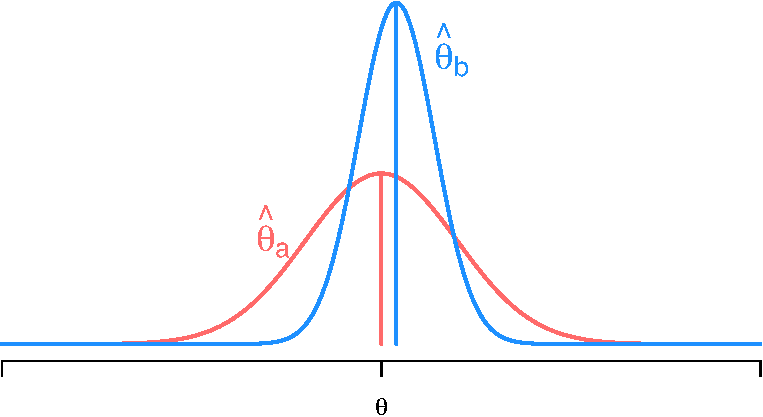
\includegraphics{./02_estimation_files/figure-pdf/mse-1.pdf}

}

\caption{Two sampling distributions}

\end{figure}

In this figure, we show the sampling distributions of two estimators,
\(\widehat{\theta}_a\), which is unbiased (centered on the true value
\(\theta\)) but with a high sampling variance, and
\(\widehat{\theta}_b\) which is slightly biased but with much lower
sampling variance. Even though \(\widehat{\theta}_b\) is biased, the
probability of drawing a value close to the truth is higher than for
\(\widehat{\theta}_a\). This balancing between bias and variance is
precisely what the MSE helps capture and, indeed, in this case,
\(MSE[\widehat{\theta}_b] < MSE[\widehat{\theta}_a]\).

\bookmarksetup{startatroot}

\hypertarget{asymptotics}{%
\chapter{Asymptotics}\label{asymptotics}}

\hypertarget{introduction-2}{%
\section{Introduction}\label{introduction-2}}

In the last chapter, we defined estimators and started to investigate
their finite-sample properties like unbiasedness and the sampling
variance. We call these ``finite-sample'' properties because
establishing them generally does not depend on the sample size. We saw
that under iid data, the sample mean is unbiased for the population
mean, but this result holds as much for \(n = 10\) as it does for
\(n = 1,000,000\). But these properties are also of limited use: we only
learn the center and spread of the sampling distribution of \(\Xbar_n\)
from these results. What about the shape of the distribution? We can
often derive the shape if we are willing to make certain assumptions on
the underlying data (for example, if the data is normal, then the sample
means will be normal as well), but this approach is brittle: if our
parametric assumption is false, we're back to square one.

In this chapter, we're going to take a different approach and see what
happens to the sampling distribution of estimators as the sample size
gets large. The study of the estimators as the sample size goes to
infinity is called \textbf{asymptotic theory}, but it's important to
understand everything we do with asymptotics will be an approximation.
No one ever has infinite data, but we hope that as our samples get
larger, the approximations will be closer to the truth. Why work in this
asymptopia, though? It turns out that many expressions are much easier
to derive in the limit than in finite samples.

\hypertarget{why-convergence-with-probability-is-hard}{%
\section{Why convergence with probability is
hard}\label{why-convergence-with-probability-is-hard}}

It's helpful to review the basic idea of convergence in deterministic
sequences from calculus:

\leavevmode\vadjust pre{\hypertarget{def-limit}{}}%
\begin{definition}[]\label{def-limit}

A sequence \(\{a_n: n = 1, 2, \ldots\}\) has the \textbf{limit} \(a\)
written \(a_n \rightarrow a\) as \(n\rightarrow \infty\) of
\(\lim_{n\rightarrow \infty} a_n = a\) if for all \(\epsilon > 0\) there
is some \(n_{\epsilon} < \infty\) such that for all
\(n \geq n_{\epsilon}\), \(|a_n - a| \leq \epsilon\).

\end{definition}

We say that \(a_n\) \textbf{converges} to \(a\) if
\(\lim_{n\rightarrow\infty} a_n = a\). Basically, a sequence converges
to a number if the sequence gets closer and closer to that number as the
sequence goes on.

Can we apply this same idea to sequences of random variables (like
estimators)? Let's look at a few examples that might help clarify the
difficult in doing so.\footnote{Due to Wasserman (2004), Chapter 5.}
Let's say that we have a sequence of \(a_n = a\) for all \(n\) (that is,
a constant sequence). Then obviously
\(\lim_{n\rightarrow\infty} a_n = a\). Now let's say we have a sequence
of random variables, \(X_1, X_2, \ldots\), that are all independent with
a standard normal distribution, \(N(0,1)\). From the analogy to the
deterministic case, it is tempting to say that \(X_n\) converges to
\(X \sim N(0, 1)\), but notice that because they are all different
random variables, \(\P(X_n = X) = 0\). Thus, we need to be careful about
saying how one variable converges to another variable.

Another example highlights subtle problems with a sequence of random
variables converging to a single value. Suppose we have a sequence of
random variables \(X_1, X_2, \ldots\) where \(X_n \sim N(0, 1/n)\).
Clearly, \(X_n\) will be concentrated around 0 for large values of
\(n\), so it is tempting to say that \(X_n\) converges to 0. But notice
that \(\P(X_n = 0) = 0\) because of the nature of continuous random
variables.

\hypertarget{convergence-in-probability-and-consistency}{%
\section{Convergence in probability and
consistency}\label{convergence-in-probability-and-consistency}}

There are several different ways that a sequence of random variance can
converge. The first type of convergence deals with sequence converging
to a single value.\footnote{Technically, a sequence can also convergence
  in probability to another random variable, but the use case of
  converging to a single number is much more commonly used in evaluating
  estimators.}

\leavevmode\vadjust pre{\hypertarget{def-inprob}{}}%
\begin{definition}[]\label{def-inprob}

A sequence of random variables, \(X_1, X_2, \ldots\), is said to
\textbf{converge in probability} to a value \(b\) if for every
\(\varepsilon > 0\), \[
\P(|X_n - b| > \varepsilon) \rightarrow 0,
\] as \(n\rightarrow \infty\). We write this \(X_n \inprob b\).

\end{definition}

With deterministic sequences, we said that \(a_n\) converges to \(a\) is
it gets closer and closer to \(a\) as \(n\) gets bigger. For convergence
in probability, the sequence of random variables converges to \(b\) is
the probability that random variables are far away from \(b\) get
smaller and smaller as \(n\) gets big.

\begin{tcolorbox}[enhanced jigsaw, title=\textcolor{quarto-callout-note-color}{\faInfo}\hspace{0.5em}{Notation alert}, breakable, titlerule=0mm, opacityback=0, rightrule=.15mm, bottomrule=.15mm, colframe=quarto-callout-note-color-frame, coltitle=black, colbacktitle=quarto-callout-note-color!10!white, bottomtitle=1mm, toptitle=1mm, colback=white, arc=.35mm, opacitybacktitle=0.6, toprule=.15mm, leftrule=.75mm, left=2mm]

You will sometimes see convergence in probability written as
\(\text{plim}(Z_n) = b\) if \(Z_n \inprob b\), \(\text{plim}\) stands
for ``probability limit.''

\end{tcolorbox}

Convergence in probability is incredibly useful for evaluating
estimators. While we said that unbiasedness was not the be all and end
all of properties of estimators, the following property is a fairly
basic and fundamental property that we would like all good estimators to
have.

\leavevmode\vadjust pre{\hypertarget{def-consistency}{}}%
\begin{definition}[]\label{def-consistency}

An estimator is \textbf{consistent} if
\(\widehat{\theta}_n \inprob \theta\).

\end{definition}

Consistency of an estimator implies that the sampling distribution of
this estimator ``collapses'' on the true value as the sample size gets
large. We say an estimator is inconsistent if it converges in
probability to any other value, which is obviously a very bad property
of an estimator. It means that as the sample size gets large, the
probability that the estimator will be close to the truth will approach
0.

We can also define convergence in probability for a sequence of random
vectors, \(\X_1, \X_2, \ldots\), where
\(\X_i = (X_{i1}, \ldots, X_{ik})\) is a random vector of length \(k\).
This sequence convergences in probbaility to a vector
\(\mb{b} = (b_1, \ldots, b_k)\) if and only if each random variable in
the vector converges to the corresponding element in \(\mb{b}\), or that
\(X_{nj} \inprob b_j\) for all \(j = 1, \ldots, k\).

\hypertarget{useful-inequalities}{%
\section{Useful inequalities}\label{useful-inequalities}}

At first glance, it appears establishing consistency of an estimator
will be difficult. How can we know if a distribution will collapse to a
specific value without knowing the shape or family of the distribution?
It turns out that there are certain relationships between the mean and
variance of a random variable and certain probability statements that
hold for all distributions (that have finite variance at least). This
will be incredibly helpful to us.

\leavevmode\vadjust pre{\hypertarget{thm-markov}{}}%
\begin{theorem}[Markov Inequality]\label{thm-markov}

For any r.v. \(X\) and any \(\delta >0\), \[
\P(|X| \geq \delta) \leq \frac{\E[|X|]}{\delta}.
\]

\end{theorem}

\begin{proof}

Notice that we can let \(Y = |X|/\delta\) and rewrite the statement as
\(\P(Y \geq 1) \leq \E[Y]\) (since \(E[|X|]/\delta = \E[|X|/\delta]\) by
the properties of expectation), which is what we will show. But notice
that \[
\mathbb{1}(Y \geq 1) \leq Y.
\] Why does this hold? We can investigate the two possible values of the
indicator function to see. If \(Y\) is less than 1, then the indicator
function will be 0, but \(Y\) is non-negative so we know that it must be
at least as big as 0 so that inequality holds. If \(Y \geq 1\) then the
indicator function 1 but we just said that \(Y \geq 1\) so the
inequality holds. If we take the expectation of both sides of this
inequality, we obtain the result (remember the expectation of an
indicator function is the probability of the event being indicated).

\end{proof}

In words, Markov's inequality says that the probability of a random
variable being large in magnitude cannot be high if the average is not
large in magnitude. Blitzstein and Hwang 2019) provide a nice intuition
behind this result. Let \(X\) be the income of a randomly selected
individual in a population and set \(\delta = 2\E[X]\), so that the
inequality becomes \(\P(X > 2\E[X]) < 1/2\) (assuming that all income is
nonnegative). Here, the inequality says that the share of the population
that has an income twice the average must be less than 0.5, since if
more than half the population was making twice the average income then
the average would have to be higher.

It's quite astounding how general this result is since it holds for all
random variables. Of course, its generality comes at the expense of not
being very informative. If \(\E[|X|] = 5\), for instance, the inequality
tells us that \(\P(|X| \geq 1) \leq 5\) which is not very helpful since
we already know that probabilities are less than 1! If we are willing to
make some assumptions about \(X\), we can get tighter bounds.

\leavevmode\vadjust pre{\hypertarget{thm-chebyshev}{}}%
\begin{theorem}[Chebyshev Inequality]\label{thm-chebyshev}

Suppose that \(X\) is r.v. for which \(\V[X] < \infty\). Then, for every
real number \(\delta > 0\), \[
\P(|X-\E[X]| \geq \delta) \leq \frac{\V[X]}{\delta^2}.
\]

\end{theorem}

\begin{proof}

To prove this, we only need to square both sides of the inequality
inside the probability statement and apply Markov's inequality: \[
\P\left( |X - \E[X]| \geq \delta \right) = \P((X-\E[X])^2 \geq \delta^2) \leq \frac{\E[(X - \E[X])^2]}{\delta^2} = \frac{\V[X]}{\delta^2},
\] with the last equality holding by the definition of variance.

\end{proof}

This is a straightforward extension of the Markov result: the
probability of a random variable being far away from its mean (that is,
\(|X-\E[X]|\) being large) is limited by the variance of the random
variable. If we let \(\delta = c\sigma\), where \(\sigma\) is the
standard deviation of \(X\), then we can use this result to bound the
normalized: \[
\P\left(\frac{|X - \E[X]|}{\sigma} > c \right) \leq \frac{1}{c^2}.
\] This says that the probability of being, say, 2 standard deviations
away from the mean must be less than 1/4 = 0.25. Notice that this bound
can be quite wide. If \(X\) is normally distributed, then we know that
just about 5\% of draws will be greater than 2 SDs away from the mean,
which is much lower than the 25\% bound implied by Chebyshev's
inequality.

\hypertarget{the-law-of-large-numbers}{%
\section{The law of large numbers}\label{the-law-of-large-numbers}}

We can now use these inequalities to show how certain estimators are
consistent for certain quantities of interest. Why are these
inequalities useful for this purpose? Remember that convergence in
probability was about the probability of an estimator being far away
from a value going to zero. Chebyshev's inequality shows that we can
bound these exact probabilities.

The most famous consistency result has a special name.

\leavevmode\vadjust pre{\hypertarget{thm-lln}{}}%
\begin{theorem}[Weak Law of Large Numbers]\label{thm-lln}

Let \(X_1, \ldots, X_n\) be a an i.i.d. draws from a distribution with
mean \(\mu = \E[X_i]\) and variance \(\sigma^2 = \V[X_i] < \infty\). Let
\(\Xbar_n = \frac{1}{n} \sum_{i =1}^n X_i\). Then,
\(\Xbar_n \inprob \mu\).

\end{theorem}

\begin{proof}

Recall that the sample mean is unbiased, so \(\E[\Xbar_n] = \mu\) with
sampling variance \(\sigma^2/n\). We can then simply apply Chebyshev to
the sample mean to get \[
\P(|\Xbar_n - \mu| \geq \delta) \leq \frac{\sigma^2}{n\delta^2}
\] An \(n\rightarrow\infty\), the right-hand side goes to 0 which means
that the left-hand side also must go to 0 which is the definition of
\(\Xbar_n\) converging in probability to \(\mu\).

\end{proof}

The weak law of large numbers (WLLN) shows that, under general
conditions, the sample mean gets closer to the population mean as
\(n\rightarrow\infty\). In fact, this result holds even when the
variance of the is infinite, though that's a situation that most
analysts will rarely face.

\begin{tcolorbox}[enhanced jigsaw, title=\textcolor{quarto-callout-note-color}{\faInfo}\hspace{0.5em}{Note}, breakable, titlerule=0mm, opacityback=0, rightrule=.15mm, bottomrule=.15mm, colframe=quarto-callout-note-color-frame, coltitle=black, colbacktitle=quarto-callout-note-color!10!white, bottomtitle=1mm, toptitle=1mm, colback=white, arc=.35mm, opacitybacktitle=0.6, toprule=.15mm, leftrule=.75mm, left=2mm]

The naming of the ``weak'' law of large numbers seems to imply the
existence of a ``strong'' law of large numbers (SLLN) and this is true.
The SLLN states that the sample mean converges to the population mean
with probability 1. This type of convergence, called \textbf{almost sure
convergence}, is stronger than convergence in probability which only
says that the probability of the sample mean being close to the
population mean converges to 1. While it is nice to know that this
stronger form of convergence holds for the sample mean under the same
assumptions, it is very rare for folks outside of theoretical
probability and statistics to need to rely on almost sure convergence.

\end{tcolorbox}

\leavevmode\vadjust pre{\hypertarget{exm-lln}{}}%
\begin{example}[]\label{exm-lln}

It can be helpful to see how the distribution of the sample mean changes
as a function of the sample size to appreciate the WLLN. We can show
this by taking repeated iid samples of different sizes from an
exponential rv with rate 0.5 so that \(\E[X_i] = 2\). In
Figure~\ref{fig-lln-sim}, we show the distribution of the sample mean
(across repeated samples) when the sample size is 15 (black), 30
(violet), 100 (blue), and 1000 (green). What we can see is how the
distribution of the sample mean is ``collapsing'' on the true population
mean, 2. The probability of being far away from 2 becomes progressively
smaller.

\begin{figure}

{\centering 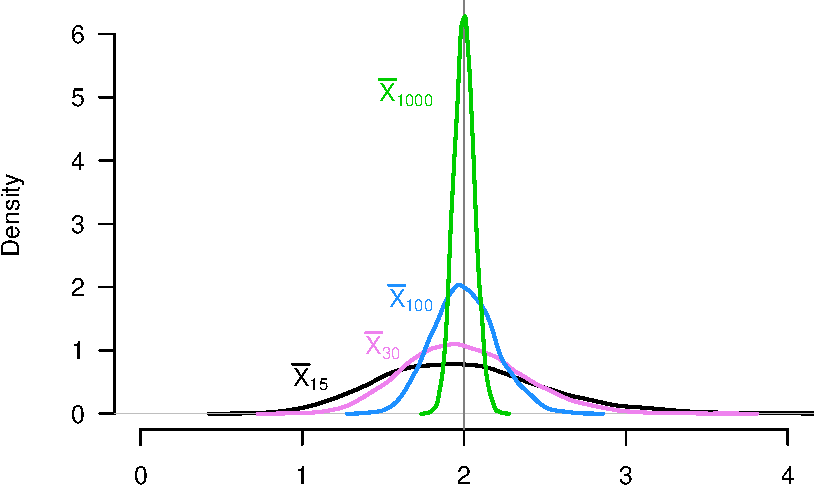
\includegraphics{./03_asymptotics_files/figure-pdf/fig-lln-sim-1.pdf}

}

\caption{\label{fig-lln-sim}Sampling distribution of the sample mean as
a function of sample size}

\end{figure}

\end{example}

The WLLN also holds for random vectors in addition to random variables.
Let \((\X_1, \ldots, \X_n)\) be an iid sample of random vectors of
length \(k\), \(\mb{X}_i = (X_{i1}, \ldots, X_{ik})\). We can define the
vector sample mean as just the vector of sample means for each of the
entries:

\[
\overline{\mb{X}}_n = \frac{1}{n} \sum_{i=1}^n \mb{X}_i =
\begin{pmatrix}
\Xbar_{n,1} \\ \Xbar_{n,2} \\ \vdots \\ \Xbar_{n, k}
\end{pmatrix}
\] Since this is just a vector of sample means, each random variable in
the random vector will converge in probability to the mean of that
random variable. Fortunately, this is the exact definition of
convergence in probability for random vectors. We formally write this in
the following theorem.

\leavevmode\vadjust pre{\hypertarget{thm-vector-wlln}{}}%
\begin{theorem}[]\label{thm-vector-wlln}

If \(\X_i \in \mathbb{R}^k\) are iid draws from a distribution with
\(\E[X_{ij}] < \infty\) for all \(j=1,\ldots,k\) then as
\(n\rightarrow\infty\)

\[
\overline{\mb{X}}_n \inprob \E[\X]  =
\begin{pmatrix}
\E[X_{i1}] \\ \E[X_{i2}] \\ \vdots \\ \E[X_{ik}]
\end{pmatrix}.
\]

\end{theorem}

\begin{tcolorbox}[enhanced jigsaw, title=\textcolor{quarto-callout-note-color}{\faInfo}\hspace{0.5em}{Notation alert}, breakable, titlerule=0mm, opacityback=0, rightrule=.15mm, bottomrule=.15mm, colframe=quarto-callout-note-color-frame, coltitle=black, colbacktitle=quarto-callout-note-color!10!white, bottomtitle=1mm, toptitle=1mm, colback=white, arc=.35mm, opacitybacktitle=0.6, toprule=.15mm, leftrule=.75mm, left=2mm]

You will have noticed that many of the formal results we have presented
so far have ``moment conditions'' that certain moments are finite. For
the vector WLLN, we saw that applied to the mean of each variable in the
vector. Some books use a short hand for this:
\(\E\Vert \X_i\Vert < \infty\), where \[
\Vert\X_i\Vert = \left(X_{i1}^2 + X_{i2}^2 + \ldots + X_{ik}^2\right)^{1/2}. 
\] This is slightly more compact notation, but why does it work? One can
show that this function, called the \textbf{Euclidean norm} or
\(L_2\)-norm is a \textbf{convex} function, so we can apply Jensen's
inequality to show that: \[
\E\Vert \X_i\Vert \geq \Vert \E[\X_i] \Vert = (\E[X_{i1}]^2 + \ldots + \E[X_{ik}]^2)^{1/2}.
\] So if \(\E\Vert \X_i\Vert\) is finite, it means that all the
component means are finite otherwise the right-hand side of the previous
equation would be infinite.

\end{tcolorbox}

\hypertarget{consistency-of-estimators}{%
\section{Consistency of estimators}\label{consistency-of-estimators}}

The WLLN shows that the sample mean of iid draws is consistent for the
population mean, which is a massive result given that so many estimators
can be written as sample means. What about other estimators? The proof
of the WLLN points to one way to determine if an estimator is
consistent: if it is unbiased and the sampling variance shrinks as the
sample size grows. The next theorem

\leavevmode\vadjust pre{\hypertarget{thm-consis}{}}%
\begin{theorem}[]\label{thm-consis}

For any estimator \(\widehat{\theta}_n\), if
\(\text{bias}[\widehat{\theta}_n] \to 0\) and
\(\V[\widehat{\theta}_n] \rightarrow 0\) as \(n\rightarrow \infty\),
then \(\widehat{\theta}_n\) is consistent.

\end{theorem}

Thus, if we can characterize the bias and sampling variance of an
estimator, then we should be able to tell if it consistent or not. This
is handy since working with the kinds of probability inequalities used
for the WLLN can sometimes be quite confusing.

What do we do if it is difficult or impossible to characterize the bias?
Consider a plug-in estimator like \(\widehat{\alpha} = \log(\Xbar_n)\)
where \(X_1, \ldots, X_n\) are iid from a population with mean \(\mu\).
We know that for nonlinear functions like logarithms we have
\(\log\left(\E[Z]\right) \neq \E[\log(Z)]\), so
\(\E[\widehat{\alpha}] \neq \log(\E[\Xbar_n])\) and the plug-in
estimator will be biased for \(\log(\mu)\). It will also be difficult to
obtain an expression for the bias in terms of \(n\). Is all hope lost
here? Must we give up on consistency? No, and in fact, consistency will
be much simpler to show in this setting.

\leavevmode\vadjust pre{\hypertarget{thm-inprob-properties}{}}%
\begin{theorem}[Properties of convergence in
probability]\label{thm-inprob-properties}

Let \(X_n\) and \(Z_n\) be two sequences of random variables such that
\(X_n \inprob a\) and \(Z_n \inprob b\), and let \(g(\cdot)\) be a
continuous function. Then,

\begin{enumerate}
\def\labelenumi{\arabic{enumi}.}
\tightlist
\item
  \(g(X_n) \inprob g(a)\) (continuous mapping theorem)
\item
  \(X_n + Z_n \inprob a + b\)
\item
  \(X_nZ_n \inprob ab\)
\item
  \(X_n/Z_n \inprob a/b\) if \(b > 0\).
\end{enumerate}

\end{theorem}

We can now see that many of the nasty problems with expectations and
nonlinear functions are made considerably easier with convergence in
probability in the asymptotic setting. So while we know that
\(\log(\Xbar_n)\) is biased for \(\log(\mu)\), we know that it is
consistent since \(\log(\Xbar_n) \inprob \log(\mu)\) because \(\log\) is
a continuous function.

\leavevmode\vadjust pre{\hypertarget{exm-nonresponse}{}}%
\begin{example}[]\label{exm-nonresponse}

Suppose we implemented a survey by randomly selecting a sample from the
population of size \(n\), but not everyone responded to our survey. Let
the data consist of pairs of random variables,
\((Y_1, R_1), \ldots, (Y_n, R_n)\), where \(Y_i\) is the question of
interest and \(R_i\) is a binary indicator for if the respondent
answered the question (\(R_i = 1\)) or not (\(R_i = 0\)). Our goal is to
estimate the mean of the question for responders:
\(\E[Y_i \mid R_i = 1]\). We can use the law of iterated expectation to
which we can rewrite as \[
\begin{aligned}
\E[Y_iR_i] &= \E[Y_i \mid R_i = 1]\P(R_i = 1) + \E[ 0 \mid R_i = 0]\P(R_i = 0) \\
\implies \E[Y_i \mid R_i = 1] &= \frac{\E[Y_iR_i]}{\P(R_i = 1)}
\end{aligned}
\]

The relevant estimator for this quantity is the mean of the of the
outcome among those who responded, which is slightly more complicated
than a typical sample mean because the denominator is a random variable:
\[
\widehat{\theta}_n = \frac{\sum_{i=1}^n Y_iR_i}{\sum_{i=1}^n R_i}. 
\] Notice that this estimator is the ratio of two random variables. The
numerator has mean \(n\E[Y_iR_i]\) and the denominator has mean
\(n\P(R_i = 1)\). It is then tempting to say that we can take the ratio
of these means as the mean of \(\widehat{\theta}_n\), but expectations
are not preserved in nonlinear functions like this one.

We can establish consistency of our estimator, though, by noting that we
can rewrite the estimator as a ratio of sample means \[
\widehat{\theta}_n = \frac{(1/n)\sum_{i=1}^n Y_iR_i}{(1/n)\sum_{i=1}^n R_i},
\] where by the WLLN the numerator
\((1/n)\sum_{i=1}^n Y_iR_i \inprob \E[Y_iR_i]\) and the denominator
\((1/n)\sum_{i=1}^n R_i \inprob \P(R_i = 1)\). Thus, by
Theorem~\ref{thm-inprob-properties}, we have \[
\widehat{\theta}_n = \frac{(1/n)\sum_{i=1}^n Y_iR_i}{(1/n)\sum_{i=1}^n R_i} \inprob \frac{\E[Y_iR_i]}{\P[R_i = 1]} = \E[Y_i \mid R_i = 1]
\] so long as the probability of responding is greater than zero. This
establishes that our sample mean among responders while biased for the
conditional expectation among responders, it is consistent for that
quantity.

\end{example}

It is very important to keep the difference between unbiased and
consistent clear in your mind. There are very many silly unbiased
estimators that are inconsistent. Let's go back to our iid sample,
\(X_1, \ldots, X_n\) from a population with \(E[X_i] = \mu\). There is
nothing in the rule book against defining an estimator
\(\widehat{\theta}_{first} = X_1\) that just uses the first observation
as the estimate. This seems like an obviously silly estimator, but it is
actually unbiased since
\(\E[\widehat{\theta}_{first}] = \E[X_1] = \mu\). It is inconsistent
since the sampling variance of this estimator is just the variance of
the population distribution,
\(\V[\widehat{\theta}_{first}] = \V[X_i] = \sigma^2\), which does not
change as a function of the sample size. Generally speaking, we can
regard ``unbiased, but inconsistent'' estimators as silly and not worth
our time (along with bias and inconsistent estimators).

There are also estimators that are biased but consistent that are often
much more interesting. We already saw one such estimator in
Example~\ref{exm-nonresponse}, but there are many more. Maximum
likelihood estimators, for example, are (under some regularity
conditions) consistent for the parameters of a parametric model, but
they are often biased.

\leavevmode\vadjust pre{\hypertarget{exm-plug-in-variance}{}}%
\begin{example}[Plug-in variance estimator]\label{exm-plug-in-variance}

Last chapter, we introduced the plug-in estimator for the population
variance, \[
\widehat{\sigma}^2 = \frac{1}{n} \sum_{i=1}^n (X_i - \Xbar_n)^2,
\] which we will now show is biased but consistent. To see the bias note
that we can rewrite the sum of square deviations
\[\sum_{i=1}^n (X_i - \Xbar_n)^2 = \sum_{i=1}^n X_i^2 - n\Xbar_n. \]
Then, the expectation of the plug-in estimator is \[
\begin{aligned}
\E[\widehat{\sigma}^2] & = \E\left[\frac{1}{n}\sum_{i=1}^n X_i^2\right] - \E[\Xbar_n^2] \\
&= \E[X_i^2] - \frac{1}{n^2}\sum_{i=1}^n \sum_{j=1}^n \E[X_iX_j] \\
&= \E[X_i^2] - \frac{1}{n^2}\sum_{i=1}^n \E[X_i^2] - \frac{1}{n^2}\sum_{i=1}^n \sum_{j\neq i} \underbrace{\E[X_i]\E[X_j]}_{\text{independence}} \\
&= \E[X_i^2] - \frac{1}{n}\E[X_i^2] - \frac{1}{n^2} n(n-1)\mu^2 \\
&= \frac{n-1}{n} \left(\E[X_i^2] - \mu^2\right) \\
&= \frac{n-1}{n} \sigma^2 = \sigma^2 - \frac{1}{n}\sigma^2
\end{aligned}. 
\] Thus, we can see that the bias of the plug-in estimator is
\(-(1/n)\sigma^2\) so it slightly underestimates the variance. Nicely,
though, the bias shrinks as a function of the sample size, so according
to Theorem~\ref{thm-consis} it will be consistent so long as the
sampling variance of \(\widehat{\sigma}^2\) shrinks as a function of the
sample size, which it does (though omit that proof here). Of course,
simply multiplying this estimator by \(n/(n-1)\) will give an unbiased
and consistent estimator that is also the typical sample variance
estimator.

\end{example}

\hypertarget{convergence-in-distribution-and-the-central-limit-theorem}{%
\section{Convergence in distribution and the central limit
theorem}\label{convergence-in-distribution-and-the-central-limit-theorem}}

Convergence in probability and the law of large numbers are very useful
for understanding how our estimators will (or will not) collapse to
their estimand as the sample size increases. But what about the shape of
the sampling distribution of our estimators? For the purposes of
statistical inference, we would like to be able to make probability
statements such as \(\P(a \leq \widehat{\theta}_n \leq b)\). These types
of statements will be the basis of hypothesis testing and confidence
intervals. But in order make those types of statements, we need to know
the entire distribution of \(\widehat{\theta}_n\), not just the mean and
variance. Luckily, there are established results that will allow us to
approximate the sampling distribution of a huge swath of estimators when
our sample sizes are large.

To see how we will develop these approximations, we need to first
describe a weaker form of convergence to a distribution rather than to a
single value.

\leavevmode\vadjust pre{\hypertarget{def-indist}{}}%
\begin{definition}[]\label{def-indist}

Let \(X_1,X_2,\ldots\), be a sequence of r.v.s, and for
\(n = 1,2, \ldots\) let \(F_n(x)\) be the c.d.f. of \(X_n\). Then it is
said that \(X_1,X_2, \ldots\) \textbf{converges in distribution} to r.v.
\(X\) with c.d.f. \(F(x)\) if \[
\lim_{n\rightarrow \infty} F_n(x) = F(x),
\] for all values of \(x\) for which \(F(x)\) is continuous. We write
this as \(X_n \indist X\) or sometimes \(X_n ⇝ X\).

\end{definition}

Essentially, convergence in distribution means that as \(n\) gets large,
the distribution of \(X_n\) becomes more and more similar to the
distribution of \(X\), which we often call the \textbf{asymptotic
distribution} of \(X_n\) (other names include the \textbf{large-sample
distribution}). If we know that \(X_n \indist X\), then we can use the
distribution of \(X\) as an approximation to the distribution of \(X_n\)
and that distribution can be fairly accurate.

One of the most remarkable results in probability and statistics is that
a large class of estimators will converge in distribution to one
particular family of distributions: the normal. This is one reason that
we study the normal so much and why investing in building intuition
about it will pay off across many domains of applied work. We call this
broad class of results the ``central limit theorem,'' (CLT) but it would
probably be more accurate to refer to them as ``central limit theorems''
since much of statistics is devoted to showing the result in different
settings. We now present the simplest CLT for the sample mean.

\leavevmode\vadjust pre{\hypertarget{thm-clt}{}}%
\begin{theorem}[Central Limit Theorem]\label{thm-clt}

Let \(X_1, \ldots, X_n\) be i.i.d. r.v.s from a distribution with mean
\(\mu = \E[X_i]\) and variance \(\sigma^2 = \V[X_i]\). Then if
\(\E[X_i^2] < \infty\), we have \[
\frac{\Xbar_n - \mu}{\sqrt{\V[\Xbar_n]}} = \frac{\sqrt{n}\left(\Xbar_n - \mu\right)}{\sigma} \indist \N(0, 1).
\]

\end{theorem}

In words: the sample mean of a random sample from a population with
finite mean and variance will be approximately normally distributed in
large samples. Notice how we have not made any assumptions about the
distribution of the underlying random variables, \(X_i\). They could
binary, event count, continuous, anything. This means the CLT is
incredibly broadly applicable.

\begin{tcolorbox}[enhanced jigsaw, title=\textcolor{quarto-callout-note-color}{\faInfo}\hspace{0.5em}{Notation alert}, breakable, titlerule=0mm, opacityback=0, rightrule=.15mm, bottomrule=.15mm, colframe=quarto-callout-note-color-frame, coltitle=black, colbacktitle=quarto-callout-note-color!10!white, bottomtitle=1mm, toptitle=1mm, colback=white, arc=.35mm, opacitybacktitle=0.6, toprule=.15mm, leftrule=.75mm, left=2mm]

Why do we state the CLT in terms of the sample mean after centering and
scaling by its standard error? If we don't normalize the sample mean in
this way, it's difficult to talk about convergence in distribution
because we know from the WLLN that \(\Xbar_n \inprob \mu\) so in the
limit the distribution of \(\Xbar_n\) is concentrated at point mass
around that value. Normalizing by centering and rescaling ensures that
the variance of the resulting quantity will be fixed as a function of
\(n\), so it makes sense to talk about its distribution converging.
Sometimes you will see the equivalent result as \[
\sqrt{n}\left(\Xbar_n - \mu\right) \indist \N(0, \sigma^2).
\]

\end{tcolorbox}

We can use this result to state approximations that we can use when
discussing estimators such as \[
\Xbar_n \overset{a}{\sim} N(\mu, \sigma^2/n),
\] where we use \(\overset{a}{\sim}\) to be ``approximately distributed
as in large samples.'' This allow us to say things like: ``in large
samples, we should expect the sample mean to between within
\(2\sigma/\sqrt{n}\) of the true mean in 95\% of repeated samples.'' As
you might guess, this will be very important for hypothesis tests and
confidence intervals! Estimators so often follow the CLT that we have an
expression for this property.

\leavevmode\vadjust pre{\hypertarget{def-asymptotically-normal}{}}%
\begin{definition}[]\label{def-asymptotically-normal}

An estimator \(\widehat{\theta}_n\) is \textbf{asymptotically normal} if
for some \(\theta\) \[
\sqrt{n}\left( \widehat{\theta}_n - \theta \right) \indist N\left(0,\V[\widehat{\theta}_n]\right).
\]

\end{definition}

\leavevmode\vadjust pre{\hypertarget{exm-bin-clt}{}}%
\begin{example}[]\label{exm-bin-clt}

To illustrate how the CLT works, we can simulate the sampling
distribution of the (normalized) sample mean at different sample sizes.
Let \(X_1, \ldots, X_n\) be iid samples from a Bernoulli with
probability of success 0.25. We then draw repeated samples of size
\(n=30\) and \(n=100\) and calculate \(\sqrt{n}(\Xbar_n - 0.25)/\sigma\)
for each random sample. Figure~\ref{fig-clt} plots the density of these
two sampling distributions along with a standard normal reference. We
can see that even at \(n=30\), the rough shape of the density looks
normal, with spikes and valleys due to the discrete nature of the data
(the sample mean can only take on 31 possible values in this case). By
\(n=100\), the sampling distribution is very close to the true standard
normal.

\begin{figure}

{\centering 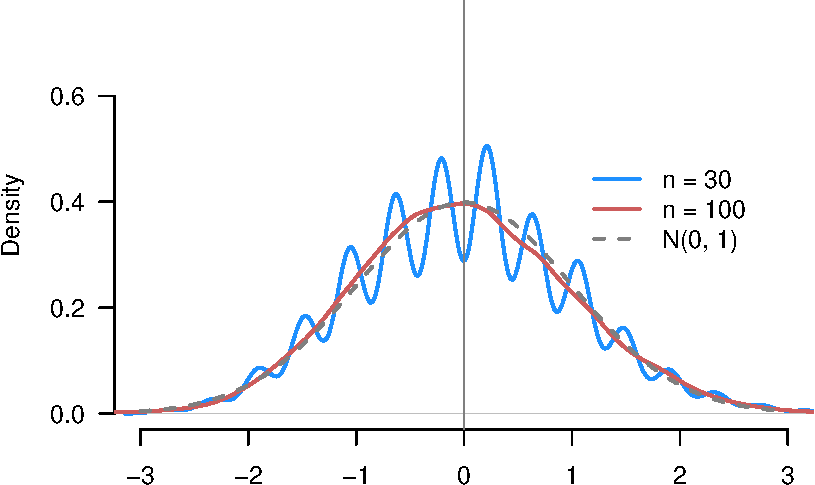
\includegraphics{./03_asymptotics_files/figure-pdf/fig-clt-1.pdf}

}

\caption{\label{fig-clt}Sampling distributions of the normalized sample
mean at n=30 and n=100.}

\end{figure}

\end{example}

There are several properties of convergence in distribution that are
helpful to us.

\leavevmode\vadjust pre{\hypertarget{thm-indist-properties}{}}%
\begin{theorem}[Properties of convergence in
distribution]\label{thm-indist-properties}

Let \(X_n\) be a sequence of random variables \(X_1,X_2,\ldots\) that
converges in distribution to some rv \(X\) and let \(Y_n\) be a sequence
of random variables \(Y_1,Y_2,\ldots\) that converges in probability to
some number, \(c\). Then,

\begin{enumerate}
\def\labelenumi{\arabic{enumi}.}
\tightlist
\item
  \(g(X_n) \indist g(X)\) for all continuous functions \(g\).
\item
  \(X_nY_n\) converges in distribution to \(cX\)
\item
  \(X_n + Y_n\) converges in distribution to \(X + c\)
\item
  \(X_n / Y_n\) converges in distribution to \(X / c\) if \(c \neq 0\)
\end{enumerate}

\end{theorem}

The last 3 of these results are sometimes referred to as
\textbf{Slutsky's theorem}. These results are very commonly used when
trying to determine the asymptotic distribution of an estimator.

One important application of Slutsky's theorem is when we replace the
(unknown) popoulation variance in the CLT with an estimate. Recall the
definition of the \textbf{sample variance} as \[
s^2 = \frac{1}{n-1} \sum_{i=1}^n (X_i - \Xbar_n)^2,
\] with the \textbf{sample standard deviation} defined as
\(s = \sqrt{s^2}\). It's easy to show that these are consistent
estimators for their respective population parameters \[ 
s^2 \inprob \sigma^2 = \V[X_i], \qquad s \inprob \sigma,
\] which by Slutsky's theorem implies that \[
\frac{\sqrt{n}\left(\Xbar_n - \mu\right)}{s} \indist \N(0, 1)
\] Comparing this result to the statement of CLT, we see that replacing
the population variance with a consistent estimate of the variance (or
standard deviation) does not affect the asymptotic distribution.

Like with the WLLN, the CLT holds for random vectors of sample means,
where their centered and scaled versions converge to a multivariate
normal distribution with a covariance matrix equal to covariance matrix
of the underlying random vectors of data, \(\X_i\).

\leavevmode\vadjust pre{\hypertarget{thm-multivariate-clt}{}}%
\begin{theorem}[]\label{thm-multivariate-clt}

If \(\mb{X}_i \in \mathbb{R}^k\) are i.i.d. and
\(\E\Vert \mb{X}_i \Vert^2 < \infty\), then as \(n \to \infty\), \[
\sqrt{n}\left( \overline{\mb{X}}_n - \mb{\mu}\right) \indist \N(0, \mb{\Sigma}),
\] where \(\mb{\mu} = \E[\mb{X}_i]\) and
\(\mb{\Sigma} = \V[\mb{X}_i] = \E\left[(\mb{X}_i-\mb{\mu})(\mb{X}_i - \mb{\mu})'\right]\).

\end{theorem}

Here, notice that \(\mb{\mu}\) is the vector of population means for all
the random variables in \(\X_i\) and \(\mb{\Sigma}\) is the
variance-covariance matrix for that vector.

\begin{tcolorbox}[enhanced jigsaw, title=\textcolor{quarto-callout-note-color}{\faInfo}\hspace{0.5em}{Note}, breakable, titlerule=0mm, opacityback=0, rightrule=.15mm, bottomrule=.15mm, colframe=quarto-callout-note-color-frame, coltitle=black, colbacktitle=quarto-callout-note-color!10!white, bottomtitle=1mm, toptitle=1mm, colback=white, arc=.35mm, opacitybacktitle=0.6, toprule=.15mm, leftrule=.75mm, left=2mm]

As with the notation alert with the WLLN, we are using a shorthand here,
\(\E\Vert \mb{X}_i \Vert^2 < \infty\), which implies that
\(\E[X_{ij}^2] < \infty\) for all \(j = 1,\ldots, k\), or equivalently,
that the variances of each variable in the sample means has finite
variance.

\end{tcolorbox}

\hypertarget{delta-method}{%
\section{Delta method}\label{delta-method}}

Suppose that we know that an estimator follows the CLT and so we have \[
\sqrt{n}\left(\widehat{\theta}_n - \theta  \right) \indist \N(0, V),
\] but we actually want to estimate \(h(\theta)\) so we use the plug-in
estimator, \(h(\widehat{\theta}_n)\). It seems like we should be able to
apply part 1 of Theorem~\ref{thm-indist-properties}, the CLT established
the large-sample distribution of the centered and scaled random
sequence, \(\sqrt{n}(\widehat{\theta}_n - \theta)\), not to the original
estimator itself like we would need to investigate the asymptotic
distribution of \(h(\widehat{\theta}_n)\). We can use a little bit of
calculus to get an approximation to the distribution we need.

\leavevmode\vadjust pre{\hypertarget{thm-delta-method}{}}%
\begin{theorem}[]\label{thm-delta-method}

If \(\sqrt{n}\left(\widehat{\theta}_n - \theta\right) \indist \N(0, V)\)
and \(h(u)\) is continuously differentiable in a neighborhood around
\(\theta\), then as \(n\to\infty\), \[
\sqrt{n}\left(h(\widehat{\theta}_n) - h(\theta)  \right) \indist \N(0, (h'(\theta))^2 V).
\]

\end{theorem}

It's useful to understand what's happening here since it might help give
intuition as to when this might go wrong. Why do we focus on
continuously differentiable functions, \(h()\)? These are functions that
can be well-approximated with a line in a neighborhood around a given
point like \(\theta\). In Figure~\ref{fig-delta}, we show this where the
tangent line at \(\theta_0\), which has slope \(h'(\theta_0)\), is very
similar to \(h(\theta)\) for values close to \(\theta_0\). Because of
this, we can approximate the difference between
\(h(\widehat{\theta}_n)\) and \(h(\theta_0)\) with the what this tangent
line would give us: \[
\underbrace{\left(h(\widehat{\theta_n}) - h(\theta_0)\right)}_{\text{change in } y} \approx \underbrace{h'(\theta_0)}_{\text{slope}} \underbrace{\left(\widehat{\theta}_n - \theta_0\right)}_{\text{change in } x},
\] and then multiplying both sides by the \(\sqrt{n}\) gives \[
\sqrt{n}\left(h(\widehat{\theta_n}) - h(\theta_0)\right) \approx h'(\theta_0)\sqrt{n}\left(\widehat{\theta}_n - \theta_0\right). 
\] The right-hand side of this approximation converges to
\(h'(\theta_0)Z\), where \(Z\) is a random variable variable with
\(\N(0, V)\). The variance of this quantity will be \[
\V[h'(\theta_0)Z] = (h'(\theta_0))^2\V[Z] = (h'(\theta_0))^2V,
\] by the properties of variances.

\begin{figure}

{\centering 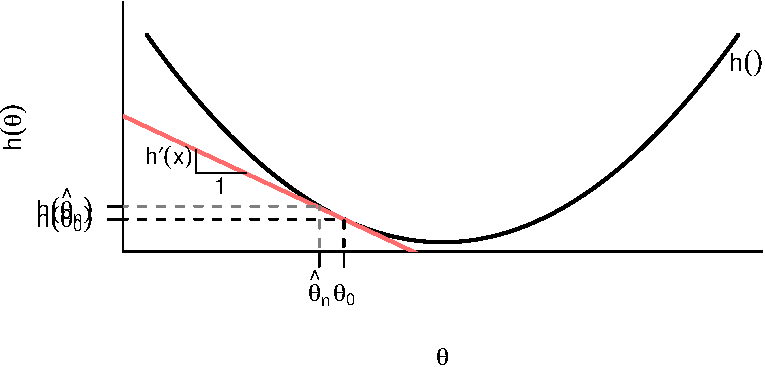
\includegraphics{./03_asymptotics_files/figure-pdf/fig-delta-1.pdf}

}

\caption{\label{fig-delta}Linear approximation to nonlinear functions}

\end{figure}

\leavevmode\vadjust pre{\hypertarget{exm-log}{}}%
\begin{example}[]\label{exm-log}

Let's return to the iid sample \(X_1, \ldots, X_n\) with mean
\(\mu = \E[X_i]\) and variance \(\sigma^2 = \V[X_i]\). From the CLT, we
know that \(\sqrt{n}(\Xbar_n - \mu) \indist \N(0, \sigma^2)\). Suppose
that we want to estimate \(\log(\mu)\) so we use the plug-in estimator
\(\log(\Xbar_n)\) (assuming that \(X_i > 0\) for all \(i\) so that we
can actually take the log). What is the asymptotic distribution of this
estimator? This is a situation where \(\widehat{\theta}_n = \Xbar_n\)
and \(h(\mu) = \log(\mu)\). From basic calculus we know that \[
h'(\mu) = \frac{\partial \log(\mu)}{\partial \mu} = \frac{1}{\mu},
\] so applying the delta method, we can determine that \[
\sqrt{n}\left(\log(\Xbar_n) - \log(\mu)\right) \indist \N\left(0,\frac{\sigma^2}{\mu^2} \right).
\]

\end{example}

\leavevmode\vadjust pre{\hypertarget{exm-exp}{}}%
\begin{example}[]\label{exm-exp}

What about if we want to estimate the \(\exp(\mu)\) with
\(\exp(\Xbar_n)\)? Recall that \[
h'(\mu) = \frac{\partial \exp(\mu)}{\partial \mu} = \exp(\mu)
\] so applying the delta method, we have \[
\sqrt{n}\left(\exp(\Xbar_n) - \exp(\mu)\right) \indist \N(0, \exp(2mu)\sigma^2),
\] since \(\exp(\mu)^2 = \exp(2\mu)\).

\end{example}

Like all of the results in this chapter, there is a multivariate version
of the delta method that is incredibly useful in practical applications.
This is because we often will take two different estimators (or two
different estimated parameters) and combine them to estimate another
quantity. We now let
\(\mb{h}(\mb{\theta}) = (h_1(\mb{\theta}), \ldots, h_m(\mb{\theta}))\)
map from \(\mathbb{R}^k \to \mathbb{R}^m\) and be continuously
differentiable (we make the function bold since it ). It will help us
use more compact matrix notation if we introduce a \(m \times k\)
Jacobian matrix of all partial derivatives \[
\mb{H}(\mb{\theta}) = \mb{\nabla}_{\mb{\theta}}\mb{h}(\mb{\theta}) = \begin{pmatrix}
  \frac{\partial h_1(\mb{\theta})}{\partial \theta_1} & \frac{\partial h_1(\mb{\theta})}{\partial \theta_2} & \cdots & \frac{\partial h_1(\mb{\theta})}{\partial \theta_k} \\
  \frac{\partial h_2(\mb{\theta})}{\partial \theta_1} & \frac{\partial h_2(\mb{\theta})}{\partial \theta_2} & \cdots & \frac{\partial h_2(\mb{\theta})}{\partial \theta_k} \\
  \vdots & \vdots & \ddots & \vdots \\
  \frac{\partial h_m(\mb{\theta})}{\partial \theta_1} & \frac{\partial h_m(\mb{\theta})}{\partial \theta_2} & \cdots & \frac{\partial h_m(\mb{\theta})}{\partial \theta_k} 
\end{pmatrix},
\] which we can use to generate the equivalent multivariate linear
approximation \[
\left(\mb{h}(\widehat{\mb{\theta}}_n) - \mb{h}(\mb{\theta}_0)\right) \approx \mb{H}(\mb{\theta}_0)'\left(\widehat{\mb{\theta}}_n - \mb{\theta}_0\right).
\] We can use this fact to derive the multivariate delta method.

\leavevmode\vadjust pre{\hypertarget{thm-multivariate-delta}{}}%
\begin{theorem}[]\label{thm-multivariate-delta}

Suppose that
\(\sqrt{n}\left(\widehat{\mb{\theta}}_n - \mb{\theta}_0 \right) \indist \N(0, \mb{\Sigma})\),
then for any function \(\mb{h}\) that is continuously differentiable in
a neighborhood of \(\mb{\theta}_0\), we have \[
\sqrt{n}\left(\mb{h}(\widehat{\mb{\theta}}_n) - \mb{h}(\mb{\theta}_0) \right) \indist \N(0, \mb{H}\mb{\Sigma}\mb{H}'), 
\] where \(\mb{H} = \mb{H}(\mb{\theta}_0)\).

\end{theorem}

This result follows from the approximation above plus rules about
variances of random vectors. Remember that for any compatible matrix of
constants, \(\mb{A}\), we have
\(\V[\mb{A}'\mb{Z}] = \mb{A}\V[\mb{Z}]\mb{A}'\). You can see that the
matrix of constants appears twice here, sort of like the matrix version
of ``squaring the constant'' rule for variance.

The delta method is a very useful for generating closed-form
approximations for asymptotic standard errors, but the math is often
quite complex for even simple estimators. For applied researchers, it is
usually more straightforward to use computational tools like the
bootstrap to approximate the standard errors we need. This has the
trade-off of taking more computational time to implement than the delta
method, but is more easily adaptable across different estimators and
domains with little human thinking time.

\bookmarksetup{startatroot}

\hypertarget{hypothesis-tests}{%
\chapter{Hypothesis tests}\label{hypothesis-tests}}

Up to now, we have discussed the properties of estimators that allow us
to sometimes characterize their distributions in finite and large
samples. These properties might allow us to say that, for example, our
estimated difference in means is equal to a true average treatment
effect on average across repeated samples or that it will converge to
the true value in large samples. These properties, however, are
properties of repeated samples whereas we as researchers will only have
access to a single sample. \textbf{Statistical inference} is the process
of using our single sample to learn about population parameters. There
are several ways to do inference that are connected, but perhaps the
most ubiquitous in the sciences is the hypothesis test, which is a kind
of statistical thought experiment.

\hypertarget{the-lady-tasting-tea}{%
\section{The lady tasting tea}\label{the-lady-tasting-tea}}

The lady tasting tea is an example of the core ideas behind hypothesis
testing due to R.A. Fisher.\footnote{Implicit in this analyis is that
  the estimate of the standard error is consistent.} Fisher had prepared
a cup of tea for his colleague, the algologist Muriel Bristol. Knowing
that she preferred milk in her tea, he poured milk into a tea cup and
then poured the hot tea into the milk. Bristol rejected the cup, stating
that she preferred the tea to be poured first, then milk. Fisher was
apparently incredulous at the idea anyone could tell the difference
between a cup poured milk-first or tea-first. So he and another
colleague, William Roach, devised a test to see if Bristol had the
ability to distinguish the two preparation methods.

For this test, Fisher and Roach prepared 8 cups of tea, 4 prepared
milk-first and 4 prepared tea-first. They then presented the cups to
Bristol in a random order (though she knew there were 4 of each type),
and she proceeded to identify all of the cups correctly. At a first
glance, this seems like good evidence that she can tell the difference
between the two types, but a skeptic like Fisher raised the question:
``could she have just been randomly guessing and got lucky?'' This led
Fisher to a \textbf{statistical thought experiment}: what would the
probability of guessing all cups correctly \emph{if} she were guessing
randomly?

To calculate the probability of Bristol's achievement, we can note that
``randomly guessing'' here would mean that she were selecting a group of
4 cups to be labeled milk-first from the 8 cups available. Using basic
combinatorics, there are 70 ways to choose 4 cups among 8, but only 1 of
those arrangements would be correct. Thus, if randomly guessing means
choosing among those 70 options with equal chance, then the probability
of guessing correctly is 1/70 or \(\approx 0.014\). This probability
being so low implies that the hypothesis of random guessing may be
implausible.

The story of the lady tasting tea encapsulates many of the core elements
of hypothesis testing. Hypothesis testing is about taking our observed
estimate (Bristol guessing all the cups correctly) and seeing how likely
that observed estimate would be under some assumption or hypothesis
about the data generating process (Bristol was randomly guessing). When
the observed estimate is very unlikely under the maintained hypothesis,
we might view this as evidence against that hypothesis. Thus, hypothesis
tests help us assess evidence for particular guesses about the DGP.

\begin{tcolorbox}[enhanced jigsaw, title=\textcolor{quarto-callout-note-color}{\faInfo}\hspace{0.5em}{Notation alert}, breakable, titlerule=0mm, opacityback=0, rightrule=.15mm, bottomrule=.15mm, colframe=quarto-callout-note-color-frame, coltitle=black, colbacktitle=quarto-callout-note-color!10!white, bottomtitle=1mm, toptitle=1mm, colback=white, arc=.35mm, opacitybacktitle=0.6, toprule=.15mm, leftrule=.75mm, left=2mm]

For the rest of this chapter, we'll introduce the concepts following the
notation in the past chapters. We'll usually assume that we have a
random (iid) sample of random variables \(X_1, \ldots, X_n\) from a
distribution, \(F\). We'll focus on estimating some parameter,
\(\theta\) of this distribution (like the mean, median, variance, etc).
We'll refer to \(\Theta\) as the set of possible values of \(\theta\),
or the \textbf{parameter space}.

\end{tcolorbox}

\hypertarget{hypotheses}{%
\section{Hypotheses}\label{hypotheses}}

In the context of hypothesis testing, hypotheses are just statements
about the population distribution. In particular, we will make
statements that \(\theta = \theta_0\) where \(\theta_0 \in \Theta\) is
the hypothesized value of \(\theta\). Hypotheses are ubiquitous in
empirical work, but here are some examples to give you a flavor:

\begin{itemize}
\tightlist
\item
  The population proportion of US citizens that identify as Democrats is
  0.33.
\item
  The population difference in average voter turnout between households
  who received receiving get-out-the-vote mailers vs those who did not
  is 0.
\item
  The difference in average incidence of human rights abuse in countries
  that signed a human rights treaty vs those countries that did not sign
  is 0.
\end{itemize}

Each of these is a statement about the true DGP. The latter two are very
common: when \(\theta\) represents the difference in means between two
groups, then \(\theta = 0\) is the hypothesis of no true difference in
population means, or no treatment effect (if the causal effect is
identified).

The goal of hypothesis testing is to adjudicate between two
complementary hypotheses.

\leavevmode\vadjust pre{\hypertarget{def-null}{}}%
\begin{definition}[]\label{def-null}

The two hypotheses in a hypothesis test are called the \textbf{null
hypothesis} and the \textbf{alternative hypothesis}, denoted as \(H_0\)
and \(H_1\), respectively.

\end{definition}

These hypotheses are complementary, so that if the null hypothesis
\(H_0: \theta \in \Theta_0\), then the alternative hypothesis is
\(H_1: \theta \in \Theta_0^c\). The ``null'' in null hypothesis might
seem odd until you realize that most hypotheses being tested are that
there is no effect of some treatment or no difference in means. For
example, suppose \(\theta\) is the difference in mean support for
expanding legal immigration between a treatment group that received a
pro-immigrant message along with some facts about immigration and a
control group that just received the factual information. Then, the
typical null hypothesis would be no difference in means or
\(H_0: \theta = 0\) and the alternative would be \(H_1: \theta \neq 0\).

There are two types of tests that differ by the form of their null and
alternative hypotheses. A \textbf{two-sided test} is of the form \[
H_0: \theta = \theta_0 \quad\text{versus}\quad H_1: \theta \neq \theta_0,
\] where the ``two-sided'' part refers to how the alternative contains
values of \(\theta\) above and below the null value \(\theta_0\). A
\textbf{one-sided test} has the form \[
H_0: \theta \leq \theta_0 \quad\text{versus}\quad H_1: \theta > \theta_0,
\] or \[
H_0: \theta \geq \theta_0 \quad\text{versus}\quad H_1: \theta < \theta_0.
\] Two-sided tests are much more common in the social science where we
want to know if there is any evidence, positive or negative, against the
presumption of no treatment effect or no relationship between two
variables. One-sided tests are for situations where we only want
evidence in one direction, which is rarely relevant to social science
research. One-sided tests also have the downside of being misused to
inflate the strength of evidence against the null and so should be
avoided. Unfortunately, the math of two-sided tests are also more
complicated.

\hypertarget{the-procedure-of-hypothesis-testing}{%
\section{The procedure of hypothesis
testing}\label{the-procedure-of-hypothesis-testing}}

At the most basic level, a \textbf{hypothesis test} is a rule that
specifies values of the sample data for which we will decide to
\textbf{reject} the null hypothesis. Let \(\mathcal{X}_n\) be the range
of the sample---that is, all possible vectors \((x_1, \ldots, x_n)\)
that have positive probability of occurring. Then, a hypothesis test
describes a region of this space, \(R \subset \mathcal{X}_n\), called
the \textbf{rejection region} where when \((X_1, \ldots, X_n) \in R\) we
will \textbf{reject} \(H_0\) and when the data is outside this region,
\((X_1, \ldots, X_n) \notin R\) we \textbf{retain}, \textbf{accept}, or
\textbf{fail to reject} the null hypothesis.\footnote{Different people
  and different textbooks describe what to do when do not reject the
  null hypothesis in different ways. The terminology is not so important
  so long as you understand that rejecting the null does not mean the
  null is logically false and ``accepting'' the null does not mean the
  null is logically true. These are simply statements about the decision
  that needs to be made as part of the hypothesis test.}

How do we decide what the rejection region should be? Even though we
define the rejection region in terms of the \textbf{sample space},
\(\mathcal{X}_n\), it's unwieldy to work with the entire vector of data.
Instead, we often formulate the rejection region in terms of a
\textbf{test statistic}, \(T = T(X_1, \ldots, X_n)\), where the
rejection region becomes \[
R = \left\{(x_1, \ldots, x_n) : T(x_1, \ldots, x_n) > c\right\},
\] where \(c\) is called the \textbf{critical value}. In words, this
says that the rejection region are the parts of the sample space that
make the test statistic sufficiently large. We reject null hypotheses
when the observed data is incompatible with those hypotheses, where the
test statistic should be a measure of this incompatibility. Note that
the test statistic is a random variable and has a distribution---we will
exploit this to understand the different properties of a hypothesis
test.

\leavevmode\vadjust pre{\hypertarget{exm-biden}{}}%
\begin{example}[]\label{exm-biden}

Suppose that \((X_1, \ldots, X_n)\) measure whether a sample of US
citizens support the current US president (\(X_i = 1\)) or not
(\(X_i = 0\)). We might be interested in the test of the null hypothesis
that the president does not have the support of a majority of American
citizens. Let \(\mu = \E[X_i] = \P(X_i = 1)\). Then, a one-sided test
would compare the two hypotheses \[ 
H_0: \mu \leq 0.5 \quad\text{versus}\quad H_1: \mu > 0.5.
\] In this case, we might use the sample mean as the test statistic, so
that \(T(X_1, \ldots, X_n) = \Xbar_n\) and we have to find some
threshold above 0.5 such that we would reject the null, \[ 
R = \left\{(x_1, \ldots, x_n): \Xbar_n > c\right\}.
\] In words, how much support should we see for the current president
before we decide to reject the notion that they lack majority support.
Below we are going to select the critical value, \(c\), to have nice
statistical properties.

\end{example}

The structure of a reject region will depend on whether a test is one-
or two-sided. One-sided tests will take the form \(T > c\), whereas
two-sided tests will take the form \(|T| > c\), since we want to count
deviations from either side of the null hypothesis as evidence against
that null.

\hypertarget{testing-errors}{%
\section{Testing errors}\label{testing-errors}}

If we are making a decision about whether to reject a null hypothesis or
not, it is possible that we will make the incorrect decision. In
particular, there are two ways for us to make errors and two ways for us
to be correct in this setting, as shown in Table~\ref{tbl-errors}. The
labels are confusing, but it's helpful to remember that \textbf{type I
errors} (said ``type one'') are labelled so because they are the worse
of the two types of errors. This is when we reject a null (say there is
a true treatment effect or relationship) when in fact the null is true
(there is no true treatment effect or relationship). Type I errors are
what we see in the replication crisis: lots of ``significant'' effects
that turn out later to be null. \textbf{Type II errors} (said ``type
two'') are considered less problematic: there is a true relationship,
but we cannot detect it with our test (cannot reject the null).

\hypertarget{tbl-errors}{}
\begin{longtable}[]{@{}lll@{}}
\caption{\label{tbl-errors}Typology of testing errors}\tabularnewline
\toprule()
& \(H_0\) True & \(H_0\) False \\
\midrule()
\endfirsthead
\toprule()
& \(H_0\) True & \(H_0\) False \\
\midrule()
\endhead
Retain \(H_0\) & Awesome & Type II error \\
Reject \(H_0\) & Type I error & Great \\
\bottomrule()
\end{longtable}

Ideally, we would minimize the chances that we make either a type I or
type II error. Unfortunately, because the test statistic is a random
variable, we cannot remove the probability of an error completely.
Instead, we will try to derive tests that have some guaranteed
performance in terms of minimizing the probability of type I error. To
derive this, we can define the \textbf{power function} of a test, \[ 
\pi(\theta) = \P\left(  \text{Reject } H_0 \mid \theta \right) = \P\left( T \in R \mid \theta \right),
\] which is the probability of rejection as a function of the parameter
of interest, \(\theta\). This tells us, for example, how likely we are
to reject the null of no treatment effect as we vary the true size of
the treatment effect.

From the power function we can define the probability of type I error.

\leavevmode\vadjust pre{\hypertarget{def-size}{}}%
\begin{definition}[]\label{def-size}

The \textbf{size} of a hypothesis test with the null hypothesis
\(H_0: \theta = \theta_0\) is \[ 
\pi(\theta_0) = \P\left( \text{Reject } H_0 \mid \theta_0 \right).
\]

\end{definition}

You can think of the size of a test as the rate of false positives (or
false discoveries) produced by the test. Figure~\ref{fig-size-power}
shows an example of rejection regions, size, and power for a one-sided
test. In the left panel, we have the distribution of the test statistic
under the null, with \(H_0: \theta = \theta_0\) and the rejection region
is defined by values \(T > c\). The shaded grey region is the
probability of rejection under this null hypothesis, or the size of the
test. Sometimes by random chance we will get samples that are extreme
even under the null, leading to false discoveries.\footnote{Eagle-eyed
  readers will notice that the null tested here is a point, where we
  previously defined the null in a one-sided test as a region
  \(H_0: \theta \leq \theta_0\). Technically, the size of the test will
  vary based on which of these nulls we pick. In this example, notice
  that any null to the left of \(\theta_0\) will result in a lower size.
  This means that the null at the boundary, \(\theta_0\) will maximize
  the size of the test and so it is the most ``conservative'' null to
  investigate. Technically, we should define the size of a test as
  \(\alpha = \sup_{\theta \in \Theta_0} \pi(\theta)\),}

In the right panel, we overlay the distribution of the test statistic
under one particular alternative, \(\theta = \theta_1 > \theta_0\). The
red shaded region is the probability of rejecting the null when this
alternative is true, or the power---it's the probability of correctly
rejecting the null when it is false. Intuitively, we can see that
alternatives that produces test statistics closer to the rejection
region will have higher power. This makes sense: it should be easier to
detect big deviations from the null than small deviations from the null.

\begin{figure}

{\centering 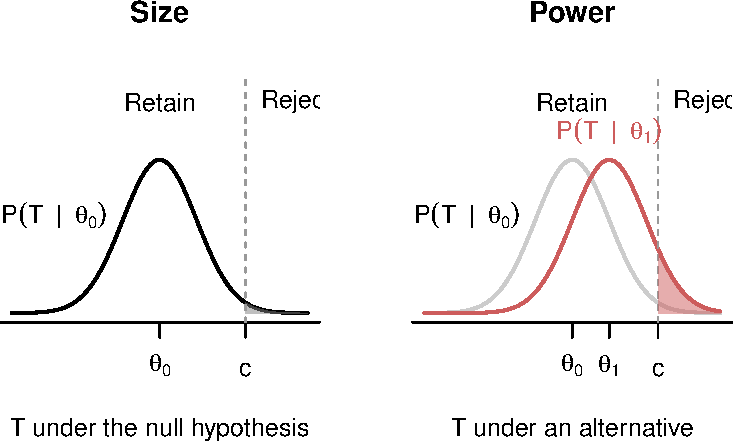
\includegraphics{./04_hypothesis_tests_files/figure-pdf/fig-size-power-1.pdf}

}

\caption{\label{fig-size-power}Size of a test and power against an
alternative}

\end{figure}

Figure~\ref{fig-size-power} also hints at a tradeoff between size and
power. Notice that we could make the size smaller (lower the false
positive rate) by increasing the critical value to \(c' > c\). This
would make the probability of being in the rejection region smaller,
\(\P(T > c' \mid \theta_0) < \P(T > c \mid \theta_0)\), leading to a
lower sized test. Unfortunately, it would also reduce power in the right
panel since the probability of being in the rejection region will be
lower under any alternative,
\(\P(T > c' \mid \theta_1) < \P(T > c \mid \theta_1)\). This means we
usually cannot simultaneously reduce both types of errors at the same
time.

\hypertarget{determining-the-rejection-region}{%
\section{Determining the rejection
region}\label{determining-the-rejection-region}}

If we cannot simultaneously optimize both the size and power of a test,
how should we determine where the reject region is? That is, how should
we determine what empirical evidence will be strong enough for us to
reject the null? The standard approach to this problem in hypothesis
testing is to control the size of a test (that is, control the rate of
false positives) and try to maximize the power of the test subject to
that constraint. So we say ``I'm willing to accept at most x\%'' of
findings will be false positives and do whatever we can to maximize
power subject to that constraint.

\leavevmode\vadjust pre{\hypertarget{def-level}{}}%
\begin{definition}[]\label{def-level}

A test has \textbf{significance level} \(\alpha\) if its size is less
than or equal to \(\alpha\), or \(\pi(\theta_0) \leq \alpha\).

\end{definition}

A test with a significance level of \(\alpha = 0.05\) means that the
test will have a false positive/type I error rate no larger than 0.05.
This is an extremely common level for tests in the social science,
though you also will \(\alpha = 0.01\) or \(\alpha = 0.1\). Frequentists
justify this by saying this means that with \(\alpha = 0.05\), there
will only 5\% of studies that will produce false discoveries.

Our task, then, is to construct the rejection region so that the
\textbf{null distribution} of the test statistic
\(G_0(t) = \P(T \leq t \mid \theta_0)\) to have less than \(\alpha\)
probability in that region. One-sided tests like in
Figure~\ref{fig-size-power} are easiest to show this even though we have
warned that you shouldn't use them. We want to choose \(c\) that puts no
more than \(\alpha\) probability in the tail, or \[ 
\P(T > c \mid \theta_0) = 1 - G_0(c) \leq \alpha.
\] Remembering that the smaller the value of \(c\) we can use will
maximize power, which implies that the critical value for the maximum
power while maintaining the significance level is when
\(1 - G_0(c) = \alpha\). We can use the \textbf{quantile function} of
the null distribution to find the exact value of \(c\) we need, \[
c = G^{-1}_0(1 - \alpha),
\] which is just fancy math to say ``the value at which \(1-\alpha\) of
the null distribution is below.''

The determination of the rejection region follows the same principles
with two-sided tests, but it is slightly more complicated because
typically need to reject when the magnitude of the test statistic is
large, \(|T| > c\). Figure~\ref{fig-two-sided} shows that basic setup.
Notice that because there are two (disjoint) regions, we can write the
size (false positive rate) as \[ 
\pi(\theta_0) = G_0(-c) + 1 - G_0(c)
\] In most cases that we will see, the null distribution for such a test
will be symmetric around 0 (usually asymptotically standard normal,
actually), which means that \(G_0(-c) = 1 - G_0(c)\), which implies that
the size is \[ 
\pi(\theta_0) = 2(1 - G_0(c)).
\] Solving for the critical value that would make this \(\alpha\) gives
\[ 
c = G^{-1}_0(1 - \alpha/2).
\] Again, this formula can seem dense, but just remember what you are
doing: finding the value that puts \(\alpha/2\) of the probability of
the null distribution in each of the tails.

\begin{figure}

{\centering 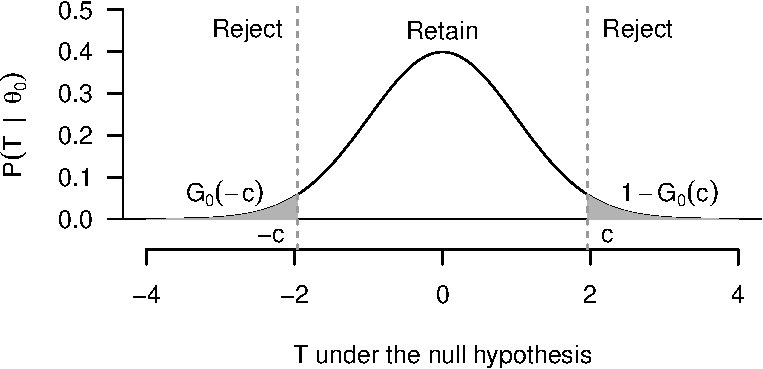
\includegraphics{./04_hypothesis_tests_files/figure-pdf/fig-two-sided-1.pdf}

}

\caption{\label{fig-two-sided}Rejection regions for a two-sided test.}

\end{figure}

\hypertarget{hypothesis-tests-of-the-sample-mean}{%
\section{Hypothesis tests of the sample
mean}\label{hypothesis-tests-of-the-sample-mean}}

Let's go through an extended example about hypothesis testing of a
sample mean, sometimes called a \textbf{one-sample test}. Let's say
\(X_i\) are feeling thermometer scores about ``liberals'' as a group on
a scale of 0 to 100, with values closer to 0 indicating cooler feelings
about liberals and values closer to 100 indicating warmer feelings about
liberals. We might want to know if the true population average is
different from a neutral value of 50. We can write this two-sided test
as \[
H_0: \mu = 50 \quad\text{versus}\quad H_1: \mu \neq 50,
\] where \(\mu = \E[X_i]\). The standard test statistic for this type of
test is the so-called \textbf{t-statistic}, \[ 
T = \frac{\left( \Xbar_n - \mu_0 \right)}{\sqrt{s^2 / n}} =\frac{\left( \Xbar_n - 50 \right)}{\sqrt{s^2 / n}},
\] where \(\mu_0\) is the null value of interest and \(s^2\) is the
sample variance. If the null hypothesis is true, then by the CLT we know
that the t-statistic is asympotically normal, \(T \indist \N(0, 1)\).
Thus, we know that the null distribution can be approximated with
standard normal!

Let's say that we want to create a test with level \(\alpha = 0.05\).
Then we need to find the rejection region that puts \(0.05\) probability
in the tails of the null distribution, which we just saw was
\(\N(0,1)\). Let \(\Phi()\) be the CDF for the standard normal and let
\(\Phi^{-1}()\) be the quantile function for the standard normal.
Drawing on what we developed above, you can find the value \(c\) so that
\(\P(|T| > c \mid \mu_0)\) is 0.05 with \[
c = \Phi^{-1}(1 - 0.05/2) \approx 1.96,
\] which means that a test where we reject when \(|T| > 1.96\) would
have a level that will be 0.05 asymptotically.

\hypertarget{the-wald-test}{%
\section{The Wald test}\label{the-wald-test}}

We can generalize the hypothesis test for the sample mean to estimators
more broadly. Let \(\widehat{\theta}_n\) be an estimator for some
parameter \(\theta\) and let
\(\widehat{\textsf{se}}[\widehat{\theta}_n]\) be a consistent estimate
of the standard error of the estimator,
\(\textsf{se}[\widehat{\theta}_n] = \sqrt{\V[\widehat{\theta}_n]}\). We
consider the two-sided test \[
H_0: \theta = \theta_0 \quad\text{versus}\quad H_1: \theta \neq \theta_0
\]

In many cases, our estimators will be asymptotically normal by a version
of the CLT. This means that under the null hypothesis, we will have \[ 
T = \frac{\widehat{\theta}_n - \theta_0}{\widehat{\textsf{se}}[\widehat{\theta}_n]} \indist \N(0, 1). 
\] The \textbf{Wald test} rejects \(H_0\) when \(|T| > z_{\alpha/2}\),
where \(z_{\alpha/2}\) that puts \(\alpha/2\) in the upper tail of the
standard normal. That is, if \(Z \sim \N(0, 1)\), then \(z_{\alpha/2}\)
satisfies \(\P(Z \geq z_{\alpha/2}) = \alpha/2\).

\begin{tcolorbox}[enhanced jigsaw, title=\textcolor{quarto-callout-note-color}{\faInfo}\hspace{0.5em}{Note}, breakable, titlerule=0mm, opacityback=0, rightrule=.15mm, bottomrule=.15mm, colframe=quarto-callout-note-color-frame, coltitle=black, colbacktitle=quarto-callout-note-color!10!white, bottomtitle=1mm, toptitle=1mm, colback=white, arc=.35mm, opacitybacktitle=0.6, toprule=.15mm, leftrule=.75mm, left=2mm]

In R, you can find the \(z_{\alpha/2}\) values easily with the
\texttt{qnorm()} function:

\begin{Shaded}
\begin{Highlighting}[]
\FunctionTok{qnorm}\NormalTok{(}\FloatTok{0.05} \SpecialCharTok{/} \DecValTok{2}\NormalTok{, }\AttributeTok{lower.tail =} \ConstantTok{FALSE}\NormalTok{)}
\end{Highlighting}
\end{Shaded}

\begin{verbatim}
[1] 1.959964
\end{verbatim}

\end{tcolorbox}

\leavevmode\vadjust pre{\hypertarget{thm-wald}{}}%
\begin{theorem}[]\label{thm-wald}

Asymptotically, the Wald test has size \(\alpha\) such that \[ 
\P(|T| > z_{\alpha/2} \mid \theta_0) \to \alpha.
\]

\end{theorem}

This is a very general result and it means that many, many hypothesis
tests based on estimators will have the same form. The main difference
across estimators will be the exact way that we calculate the estimated
standard error.

\leavevmode\vadjust pre{\hypertarget{exm-two-props}{}}%
\begin{example}[Difference in proportions]\label{exm-two-props}

In get-out-the-vote (GOTV) experiments, we might randomly assign a group
of citizens to receive mailers that encourage them to vote, whereas a
control group receives no message. We'll define the turnout variables in
the treatment group \(Y_{1}, Y_{2}, \ldots, Y_{n_t}\) as iid draws from
a Bernoulli distribution with success \(p_t\) which represents the
population turnout rate among treated citizens. The outcomes in the
control group \(X_{1}, X_{2}, \ldots, X_{n_c}\) are iid draws from
another Bernoulli distribution with success \(p_c\), which represents
the population turnout rate among citizens not receiving a mailer.

Our goal is to learn about the treatment effect of this treatment on
whether or not the citizen votes, \(\tau = p_t - p_c\) and we will use
the sample difference in means/proportions as our estimator,
\(\widehat{\tau} = \Ybar - \Xbar\). To perform a Wald test, we need to
know/estimate the standard error of this estimator. Notice that because
these are independent samples, the variance is \[ 
\V[\widehat{\tau}_n] =  \V[\Ybar - \Xbar] = \V[\Ybar] + \V[\Xbar] = \frac{p_t(1-p_t)}{n_t} + \frac{p_c(1-p_c)}{n_c},
\] where the third equality comes from the fact that the underlying
outcome variables \(Y_i\) and \(X_j\) are binary. Obviously we do not
know the true population proportions \(p_t\) and \(p_c\) (that's why
we're doing the test!), but we can estimate the standard error by
replacing them with their estimates \[ 
\widehat{\textsf{se}}[\widehat{\tau}] = \sqrt{\frac{\Ybar(1 -\Ybar)}{n_t} + \frac{\Xbar(1-\Xbar)}{n_c}}.
\]

The typical null hypothesis test in this case is ``no treatment effect''
vs ``some treatment effect'' or \[
H_0: \tau = p_t - p_c = 0 \quad\text{versus}\quad H_1: \tau \neq 0,
\] which gives the following test statistic for the Wald test \[
T = \frac{\Ybar - \Xbar}{\sqrt{\frac{\Ybar(1 -\Ybar)}{n_t} + \frac{\Xbar(1-\Xbar)}{n_c}}}. 
\] If we wanted a test with level \(\alpha = 0.01\), we would reject the
null when \(|T| > 2.58\) since

\begin{Shaded}
\begin{Highlighting}[]
\FunctionTok{qnorm}\NormalTok{(}\FloatTok{0.01}\SpecialCharTok{/}\DecValTok{2}\NormalTok{, }\AttributeTok{lower.tail =} \ConstantTok{FALSE}\NormalTok{)}
\end{Highlighting}
\end{Shaded}

\begin{verbatim}
[1] 2.575829
\end{verbatim}

\end{example}

\leavevmode\vadjust pre{\hypertarget{exm-diff-in-means}{}}%
\begin{example}[Difference in means]\label{exm-diff-in-means}

Let's take a similar setting to the last example with randomly assigned
treatment and control groups, but now the treatment is an appeal for
donations and the outcomes are continuous measures of how much a person
donated to the political campaign. Now the treatment data
\(Y_1, \ldots, Y_{n_t}\) are iid draws from a population with mean
\(\mu_t = \E[Y_i]\) and population variance \(\sigma^2_t = \V[Y_i]\).
The control data \(X_1, \ldots, X_{n_c}\) are iid draws (independent of
the \(Y_i\)) from a population with mean \(\mu_c = \E[X_i]\) and
population variance \(\sigma^2_c = \V[X_i]\). The parameter of interest
is similar to before: the population difference in means,
\(\tau = \mu_t - \mu_c\), and we'll form the usual hypothesis test of
\[ 
H_0: \tau = \mu_t - \mu_c = 0 \quad\text{versus}\quad H_1: \tau \neq 0.
\]

The only difference between this setting and the difference in
proportions is the standard error here will be different because we
cannot rely on the Bernoulli. Instead, we'll use our knowledge of the
sampling variance of the sample means and independence between the
samples to derive \[  
\V[\widehat{\tau}] = \V[\Ybar] + \V[\Xbar] = \frac{\sigma^2_t}{n_t} + \frac{\sigma^2_c}{n_c},
\] where we can come up with an estimate of the unknown population
variance with sample variances \[  
\widehat{\se}[\widehat{\tau}] = \sqrt{\frac{s^2_t}{n_t} + \frac{s^2_c}{n_c}}.
\] This leads to the Wald test statistic of \[ 
T = \frac{\widehat{\tau} - 0}{\widehat{\se}[\widehat{\tau}]} = \frac{\Ybar - \Xbar}{\sqrt{\frac{s^2_t}{n_t} + \frac{s^2_c}{n_c}}},
\] and if want an asymptotically level of 0.05, we can reject when
\(|T| > 1.96\).

\end{example}

\hypertarget{p-values}{%
\section{p-values}\label{p-values}}

The hypothesis testing framework is clearly designed for actually making
a decision in the face of uncertainty. You choose a level of wrongness
you are comfortable with (rate of false positives) and then make a
decision null vs alternative based firmly on the rejection region. This
has the downside that when we're not really making a decision, we are
somewhat artificially discarding information about the strength of
evidence. We ``accept'' the null if \(T = 1.95\) in the last example but
reject it if \(T = 1.97\) even though these two situations are actually
very similar. Just reporting the reject/retain decision also fails to
give us a sense of at what other levels we might have rejected the null.
Again, this makes sense if we need to make a single decision: other
tests don't matter because we carefully considered our \(\alpha\) level
test. But in the lower stakes world of the academic social sciences, we
can afford to be more informative.

One alternative to reporting the reject/retain decision is to report a
\textbf{p-value}.

\leavevmode\vadjust pre{\hypertarget{def-p-value}{}}%
\begin{definition}[]\label{def-p-value}

The \textbf{p-value} of a test is the probability of observing a test
statistic is at least as extreme as the observed test statistic in the
direction of the alternative hypothesis.

\end{definition}

The line about ``in the direction of the alternative hypothesis'' deals
with the unfortunate headache of one-sided versus two-sided tests. For a
one-sided test where larger values of \(T\) correspond to more evidence
for \(H_1\), the p-value is \[
\P(T(X_1,\ldots,X_n) > T \mid \theta_0) = 1 - G_0(T),
\] whereas for a (symmetric) two-sided test we have \[ 
\P(|T(X_1, \ldots, X_n)| > |T| \mid \theta_0) = 2(1 - G_0(|T|)).
\]

In either case, the interpretation of the p-value is the same. It is the
smallest size \(\alpha\) at which a test would reject null. Presenting a
p-value allows the reader to determine their own \(\alpha\) level and
determine quickly if the evidence would warrant rejecting \(H_0\) in
that case. Thus, the p-value is a more \textbf{continuous} measure of
evidence against the null, where lower values are stronger evidence
against the null because the observed result is less likely under the
null.

There is quite a bit of controversy surrounding p-values but most of it
focuses on arbitrary p-value cutoffs for determining statistical
significance and sometimes publication decisions. This really isn't the
fault of p-values, but rather the hyperfixation on the reject/retain
decision for arbitrary test levels like \(\alpha = 0.05\). It might be
best to view p-values as a transformation of the test statistic onto a
common scale between 0 and 1.

\begin{tcolorbox}[enhanced jigsaw, title=\textcolor{quarto-callout-warning-color}{\faExclamationTriangle}\hspace{0.5em}{Warning}, breakable, titlerule=0mm, opacityback=0, rightrule=.15mm, bottomrule=.15mm, colframe=quarto-callout-warning-color-frame, coltitle=black, colbacktitle=quarto-callout-warning-color!10!white, bottomtitle=1mm, toptitle=1mm, colback=white, arc=.35mm, opacitybacktitle=0.6, toprule=.15mm, leftrule=.75mm, left=2mm]

There are many statistical shibboleths that people use to purportedly
identify people that don't understand statistics and they usually hinge
on seemingly subtle differences in interpretation that are easy to miss.
If you understand the core concepts, the statistical shibboleths tend to
be overblown, but it would be malpractice not flag them for you.

The shibboleth with p-values is that sometimes people will interpret
them as ``the probability that the null hypothesis is true.'' Of course,
this doesn't make sense from our definition because the p-values
\emph{conditions} on the null hypothesis---it cannot tell us anything
about the probability of that null hypothesis. Instead, the metaphor you
should always carry is that hypothesis tests are statistical thought
experiments and that p-values answer the question: how likely would my
data be if the null were true?

\end{tcolorbox}

\hypertarget{power-analysis}{%
\section{Power analysis}\label{power-analysis}}

Imagine you have spent a large research budget on a big experiment to
test your amazing theory and the results come back and\ldots{} you fail
to reject the null of no treatment effect. When this happens, there are
two possible states of the world: the null is true and you correctly
identified that, or the null is false but the test had lower power to
detect the true effect. Because of this uncertainty after the fact, it
is common for researchers to conduct \textbf{power analyses} prior to
running studies that try to forecast what sample size is necessary to
ensure you will be able to reject the null under a hypothesized effect
size.

Generally power analyses involve calculating the power function
\(\pi(\theta) = \P(T(X_1, \ldots, X_n) \in R \mid \theta)\) for
different values of \(\theta\). It might also involve sample size
calculations for a particular alternative, \(\theta_1\). In that case,
we try to find the sample size \(n\) that would make the power
\(\pi(\theta_1)\) as close to a particular value (often 0.8) as
possible. In simple one-sided tests, it is possible to solve for this
sample size explicitly, but for more general situations or two-sided
tests, we typically need to use numerical or simulation-based approaches
to finding the optimal sample size.

With Wald tests, we can characterize the power function quite easily
even if it does not allow us to back out sample size calculations
easily.

\leavevmode\vadjust pre{\hypertarget{thm-power}{}}%
\begin{theorem}[]\label{thm-power}

For a Wald test with an asymptotically normal estimator, the power
function for a particular alternative \(\theta_1 \neq \theta_0\) is \[ 
\pi(\theta_1) = 1 - \Phi\left( \frac{\theta_0 - \theta_1}{\widehat{\se}[\widehat{\theta}_n]} + z_{\alpha/2} \right) + \Phi\left( \frac{\theta_0 - \theta_1}{\widehat{\se}[\widehat{\theta}_n]}-z_{\alpha/2} \right).
\]

\end{theorem}

\hypertarget{exact-tests-under-normal-data}{%
\section{Exact tests under normal
data}\label{exact-tests-under-normal-data}}

The Wald test above relies on large sample approximations. In finite
samples, these approximation may not be valid. Is it possible to get
\textbf{exact} inferences at any sample size? Yes, if we make stronger
assumptions about the data. In particular, assume a \textbf{parametric
model} for the data where \(X_1,\ldots,X_n\) are i.i.d. samples from
\(N(\mu,\sigma^2)\). Under null of \(H_0: \mu = \mu_0\), we can show
that \[ 
T_n = \frac{\Xbar_n - \mu_0}{s_n/\sqrt{n}} \sim t_{n-1},
\] where \$t\_\{n-1\} is the \$\textbf{Student's t-distribution} with
\(n-1\) degrees of freedom. This implies the null distribution is \(t\)
so we use quantiles of \(t\) for critical values. For one-sided test
\(c = G^{-1}_0(1 - \alpha)\) but now \(G_0\) is \(t\) with \(n-1\) df
and so we use \texttt{qt()} instead of \texttt{qnorm()} to calculate
these critical values.

The critical values for the \(t\) distribution are always larger than
the normal because the t has fatter tails as shown in
Figure~\ref{fig-shape-of-t}. As \(n\to\infty\), however, the \(t\)
converges to the standard normal and so it is asymptotically equivalent
to the Wald test but slightly more conservative in finite samples.
Oddly, most software packages calculate p-values and rejection regions
based on the \(t\) to take advantage of this conservativeness.

\begin{figure}

{\centering 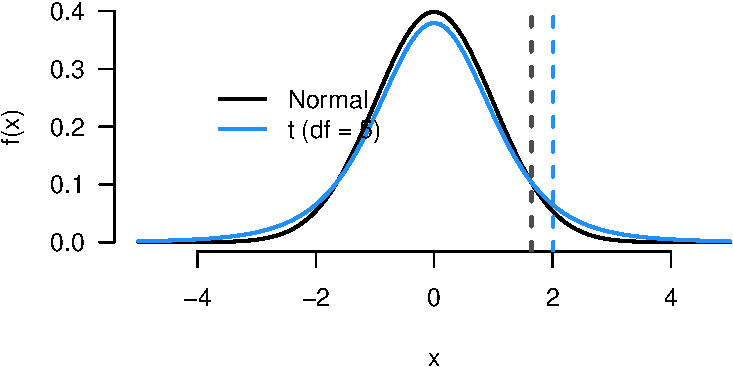
\includegraphics{./04_hypothesis_tests_files/figure-pdf/fig-shape-of-t-1.pdf}

}

\caption{\label{fig-shape-of-t}Normal versus t distribution}

\end{figure}

\bookmarksetup{startatroot}

\hypertarget{confidence-intervals}{%
\chapter{Confidence intervals}\label{confidence-intervals}}

You have run your experiment and presented your readers with your single
best guess about the treatment effect with the difference in sample
means. You may have also presented the estimated standard error of this
estimate to give readers a sense of how variable the estimate is. You
might have even done a hypothesis test against the null of no treatment
effect. But none of these approaches answer a fairly compelling
question: what range of values of the treatment effect are
\textbf{plausible} given the data we observe?

A point estimate typically has 0 probability of being the exact true
value, but intuitively we hope that the true value is close to this
estimate. \textbf{Confidence intervals} make this kind of intuition more
formal by instead estimating ranges of values with a fixed percentage of
these ranges containing the true value of the parameter.

We begin with the basic definition of a confidence interval.

\leavevmode\vadjust pre{\hypertarget{def-coverage}{}}%
\begin{definition}[]\label{def-coverage}

A \(1-\alpha\) \textbf{confidence interval} for a real-valued parameter
\(\theta\) is a pair of statistics \(L= L(X_1, \ldots, X_n)\) and
\(U = U(X_1, \ldots, X_n)\) such that \(L < U\) for all values of the
sample and such that \[ 
\P(L \leq \theta \leq U \mid \theta) \geq 1-\alpha, \quad \forall \theta \in \Theta.
\]

\end{definition}

We say that that a \(1-\alpha\) confidence intervals covers (contains,
captures, traps, etc) the true value at least \(100(1-\alpha)\%\) of the
time, and we refer to \(1-\alpha\) as the \textbf{coverage probability}
or simply \textbf{coverage}. Common confidence intervals include 95\%
percent (\(\alpha = 0.05\)) and 90\% (\(\alpha = 0.1\)).

So a confidence intervals is a random interval that has a particular
guarantee about how often it will contain the true value. It's important
to remember what is random and what is fixed in this setup. The interval
varies from sample to sample but the true value of the parameter stays
fixed, and the coverage is how often we should expect the interval to
contain that true value. The ``repeating my sample over and over again''
analogy can break down very quickly, so it's sometimes helpful to
interpret as giving guarantees across confidence intervals across
different experiments. In particular, suppose that a journal publishes
100 quantitative articles per year and each produces a single 95\%
confidence interval for their quantity of interest. Then, if the
confidence intervals are valid, then we should expect 5 of those
confidence intervals to not contain their true quantity of interest.

\begin{tcolorbox}[enhanced jigsaw, title=\textcolor{quarto-callout-warning-color}{\faExclamationTriangle}\hspace{0.5em}{Warning}, breakable, titlerule=0mm, opacityback=0, rightrule=.15mm, bottomrule=.15mm, colframe=quarto-callout-warning-color-frame, coltitle=black, colbacktitle=quarto-callout-warning-color!10!white, bottomtitle=1mm, toptitle=1mm, colback=white, arc=.35mm, opacitybacktitle=0.6, toprule=.15mm, leftrule=.75mm, left=2mm]

Let's say you calculate a 95\% confidence interval and it's
\([0.1, 0.4]\). It's tempting to make a probability statement like
\(\P(0.1 \leq \theta \leq 0.4 \mid \theta) = 0.95\) or that there's a
95\% chance that the true parameter is in \([0.1, 0.4]\). But looking at
the probability statement, everything on left-hand side of the
conditioning bar is fixed, so the probability either has to be 0
(\(\theta\) is outside the interval) or 1 (\(\theta\) is in the
interval). The coverage probability of a confidence interval refers to
its status as a pair of random variables, \((L, U)\), not any particular
realization of those variables like \((0.1, 0.4)\). As an analogy,
considering if calculated the sample mean as \(0.25\) and then tried to
say that \(0.25\) is unbiased for the population mean. This doesn't make
sense because unbiasedness refers to how the sample mean varies from
sample to sample.

\end{tcolorbox}

In most cases, we will not be able to derive exact confidence intervals,
but rather confidence intervals that are \textbf{asymptotically valid},
which means that if we write the interval as a function of the sample
size, \((L_n, U_n)\) they would have \textbf{asymptotic coverage} \[
\lim_{n\to\infty} \P(L_n \leq \theta \leq U_n) \leq 1-\alpha \quad\forall\theta\in\Theta.
\]

This will usually be the property that we can show for most confidence
intervals, since we usually rely on large sample approximations based on
the central limit theorem.

\hypertarget{deriving-confidence-intervals}{%
\section{Deriving confidence
intervals}\label{deriving-confidence-intervals}}

If you have taken any statistics before, you probably have seen the
standard formula for the 95\% confidence interval of the sample mean,
\[ 
\left[\Xbar_n - 1.96\frac{s}{\sqrt{n}},\; \Xbar_n + 1.96\frac{s}{\sqrt{n}}\right],
\] where you can recall that \(s\) is the sample standard deviation and
\(s/\sqrt{n}\) is the estimate of the standard error of the sample mean.
If this is a 95\% confidence interval, then the probability that it
contains the population mean \(\mu\) should be 0.95, but how can derive
this? It turns out that this will be justified by the central limit
theorem and we will show the logic for a generic asymptotically normal
estimator.

Let's say that we have an estimator, \(\widehat{\theta}_n\) for the
parameter \(\theta\) with estimated standard error
\(\widehat{\se}[\widehat{\theta}_n]\). If the estimator is
asymptotically normal, then in large samples, we know that \[ 
\frac{\widehat{\theta}_n - \theta}{\widehat{\se}[\widehat{\theta}_n]} \sim \N(0, 1).
\] We can then use our knowledge of the standard normal and the
empirical rule to find \[ 
\P\left( -1.96 \leq \frac{\widehat{\theta}_n - \theta}{\widehat{\se}[\widehat{\theta}_n]} \leq 1.96\right) = 0.95
\] and by multiplying each part of the inequality by
\(\widehat{\se}[\widehat{\theta}_n]\), we get \[ 
\P\left( -1.96\,\widehat{\se}[\widehat{\theta}_n] \leq \widehat{\theta}_n - \theta \leq 1.96\,\widehat{\se}[\widehat{\theta}_n]\right) = 0.95,
\] We then subtract all part by the estimator to get \[ 
\P\left(-\widehat{\theta}_n - 1.96\,\widehat{\se}[\widehat{\theta}_n] \leq  - \theta \leq -\widehat{\theta}_n + 1.96\,\widehat{\se}[\widehat{\theta}_n]\right) = 0.95,
\] and finally we multiply all parts by \(-1\) (and flipping the
inequalities) to arrive at \[ 
\P\left(\widehat{\theta}_n - 1.96\,\widehat{\se}[\widehat{\theta}_n] \leq  \theta \leq \widehat{\theta}_n + 1.96\,\widehat{\se}[\widehat{\theta}_n]\right) = 0.95.
\] To connect back to the definition of the confidence interval, we have
now shown that the random interval \([L, U]\) where \[ 
\begin{aligned}
  L = L(X_1, \ldots, X_n) &= \widehat{\theta}_n - 1.96\,\widehat{\se}[\widehat{\theta}_n] \\
  U = U(X_1, \ldots, X_n) &= \widehat{\theta}_n + 1.96\,\widehat{\se}[\widehat{\theta}_n],
\end{aligned}
\] is an asymptotically valid estimator.\footnote{Implicit in this
  analyis is that the estimate of the standard error is consistent.}
Replacing \(\Xbar_n\) for \(\widehat{\theta}_n\) and \(s/\sqrt{n}\) for
\(\widehat{\se}[\widehat{\theta}_n]\) establishes how the standard 95\%
confidence interval for the sample mean above asymptotically valid.

\begin{figure}

{\centering 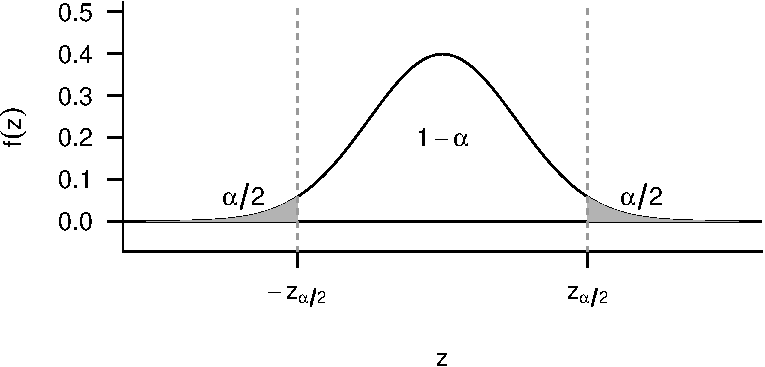
\includegraphics{./05_confidence_intervals_files/figure-pdf/fig-std-normal-1.pdf}

}

\caption{\label{fig-std-normal}Critical values for the standard normal.}

\end{figure}

How can we generalize this to \(1-\alpha\) confidence intervals? For a
standard normal rv, \(Z\), we know that \[ 
\P(-z_{\alpha/2} \leq Z \leq z_{\alpha/2}) = 1-\alpha
\] which implies that we can obtain a \(1-\alpha\) asymptotic confidence
intervals by using the interval \([L, U]\), where \[ 
L = \widehat{\theta}_{n} - z_{\alpha/2} \widehat{\se}[\widehat{\theta}_{n}], \quad U = \widehat{\theta}_{n} + z_{\alpha/2} \widehat{\se}[\widehat{\theta}_{n}]. 
\] This is sometimes shortened to
\(\widehat{\theta}_n \pm z_{\alpha/2} \widehat{\se}[\widehat{\theta}_{n}]\).
Remember that we can obtain the values of \(z_{\alpha/2}\) easily from
R:

\begin{Shaded}
\begin{Highlighting}[]
\DocumentationTok{\#\# alpha = 0.1 for 90\% CI}
\FunctionTok{qnorm}\NormalTok{(}\FloatTok{0.1} \SpecialCharTok{/} \DecValTok{2}\NormalTok{, }\AttributeTok{lower.tail =} \ConstantTok{FALSE}\NormalTok{)}
\end{Highlighting}
\end{Shaded}

\begin{verbatim}
[1] 1.644854
\end{verbatim}

As a concrete example, then, we could derive a 90\% asymptotic
confidence interval for the sample mean as \[ 
\left[\Xbar_{n} - 1.64 \frac{\widehat{\sigma}}{\sqrt{n}}, \Xbar_{n} + 1.64 \frac{\widehat{\sigma}}{\sqrt{n}}\right]
\]

\hypertarget{interpreting-confidence-intervals}{%
\section{Interpreting confidence
intervals}\label{interpreting-confidence-intervals}}

Remember that the interpretation of cofidence is how the random interval
performs over repeated samples. A valid 95\% confidence interval is a
random interval that will contain the true value in 95\% of samples.
Simulating repeated samples can help to clarify this a bit.

\leavevmode\vadjust pre{\hypertarget{exm-cis}{}}%
\begin{example}[]\label{exm-cis}

Suppose that we are taking samples of size \(n=500\) of random variables
where \(X_i \sim \N(1, 10)\), and we want to estimate the population
mean \(\E[X] = 1\). To do so, we repeat the following steps:

\begin{enumerate}
\def\labelenumi{\arabic{enumi}.}
\tightlist
\item
  Draw a sample of \(n=500\) from \(\N(1, 10)\).
\item
  Calculate the 95\% confidence interval sample mean
  \(\Xbar_n \pm 1.96\widehat{\sigma}/\sqrt{n}\).
\item
  Plot the intervals along the x-axis and color them blue if they
  contain the truth (1) and red if they do not.
\end{enumerate}

Figure~\ref{fig-ci-sim} shows 100 iteraction of these steps. Here we see
that, as expected, the large majority of calculated CIs conatain the
true value. In fact, exactly 5 of the random samples produce intervals
that fail to include 1, which is an exact coverage rate of 95\%. Of
course, this is just one simulation and a different set of 100 random
samples might have produced a slightly different coverage rate. The
gauarantee of the 95\% confidence intervals is that if we were to
continue to take these repeated samples the long-run frequency of
intervals covering the truth would approach 0.95.

\begin{figure}

{\centering 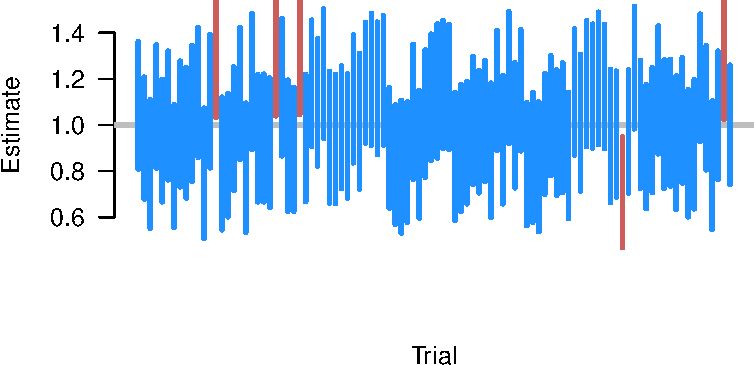
\includegraphics{./05_confidence_intervals_files/figure-pdf/fig-ci-sim-1.pdf}

}

\caption{\label{fig-ci-sim}95\% confidence intervals from 100 random
samples. Intervals are blue if they contain the truth and red if they do
not.}

\end{figure}

\end{example}

\hypertarget{confidence-intervals-and-hypothesis-tests}{%
\section{Confidence intervals and hypothesis
tests}\label{confidence-intervals-and-hypothesis-tests}}

At first glance, we may seem sloppy in using \(\alpha\) in the
derivation of a \(1 - \alpha\) confidence interval in this chapter and
in an \(\alpha\)-level test in the last chapter. In reality, we were
simply foreshadowing the deep connection between the two: every
\(1-\alpha\) confidence interval contains all null hypotheses that we
\textbf{would not reject} with an \(\alpha\)-level test.

This connection is easiest to see with a asymptotically normal
estimator, \(\widehat{\theta}_n\). Consider the hypothesis test of \[ 
H_0: \theta = \theta_0 \quad \text{vs.}\quad H_1: \theta \neq \theta_0,
\] using the test statistic, \[ 
T = \frac{\widehat{\theta}_{n} - \theta_{0}}{\widehat{\se}[\widehat{\theta}_{n}]}. 
\] As we discussed in the last chapter, an \(\alpha = 0.05\) test would
reject this null when \(|T| > 1.96\), or when \[ 
|\widehat{\theta}_{n} - \theta_{0}| > 1.96 \widehat{\se}[\widehat{\theta}_{n}]. 
\] Notice that will be true when \[ 
\theta_{0} < \widehat{\theta}_{n} - 1.96\widehat{\se}[\widehat{\theta}_{n}]\quad \text{ or  }\quad  \widehat{\theta}_{n} +  \widehat{\se}[\widehat{\theta}_{n}] < \theta_{0}
\] or, equivalently, that null hypothesis is outside of the 95\%
confidence interval,
\[\theta_0 \notin \left[\widehat{\theta}_{n} - 1.96\widehat{\se}[\widehat{\theta}_{n}], \widehat{\theta}_{n} + 1.96\widehat{\se}[\widehat{\theta}_{n}]\right].\]
Of course, our choice of the null hypothesis was arbitrary, which means
that any null hypothesis that is outside the 95\% confidence interval
would be rejected by a \(\alpha = 0.05\) level test of that null. And
any null hypothesis inside the confidence interval is a null hypothesis
that we would not reject.

This relationship holds more broadly. Any \(1-\alpha\) confidence
interval contains all possible parameter values that would not be
rejected as the null hypothesis of an \(\alpha\)-level hypothesis test.
This can be really useful for two reasons:

\begin{enumerate}
\def\labelenumi{\arabic{enumi}.}
\tightlist
\item
  We can quickly determine if a null hypothesis is rejected at some
  level by inspecting if it falls in a confidence interval.
\item
  There are situations where determining a confidence interval might be
  difficult, but performing a hypothesis test is straightforward. Then,
  we can find the rejection region for the test and determine what null
  hypotheses would not be rejected at level \(\alpha\) to formulate the
  \(1-\alpha\) confidence interval. This process is called
  \textbf{inverting a test}. One important application of this method is
  for formulating confidence intervals for treatment effects based on
  randomization inference in the finite population analysis of
  experiments.
\end{enumerate}

\bookmarksetup{startatroot}

\hypertarget{linear-regression}{%
\chapter{Linear regression}\label{linear-regression}}

Regression refers to a collection of tools for assessing the
relationship between a \textbf{outcome variable}, \(Y_i\), and a set of
\textbf{covariates}, \(\X_i\). In particular, these tools focus on
showing how the conditional mean of \(Y_i\) varies as a function
\(\X_i\). For example, we may want to know how wait voting poll wait
times vary as a function of some socioeconomic features of the precinct
like income and racial composition. This is usually accomplished by
estimating the \textbf{regression function} or \textbf{conditional
expectation function} (CEF) of the outcome given the covariates, \[
\mu(\bfx) = \E[Y_i \mid \X_i = \bfx].
\] Why is estimation and inference for this regression function special?
Why can't we just use the approaches we have seen for the mean,
variance, covariance, and so on? The basic problem with the CEF is that
there may be many, many values \(\bfx\) that can occur and so many, many
different conditional expectations that we will need to estimate. In
fact, if any variable in \(\X_i\) is continuous, then there will be an
infinite number of possible values of \(\bfx\) that we need to estimate.
Because this problem gets worse as we add covariates to \(\X_i\), this
is sometimes referred to as the \textbf{curse of dimensionality}. How
can we resolve this with our measely finite data?

In this chapter, we are going to explore two different ways of
``solving'' the curse of dimensionality: assuming it away and changing
the quantity of interest to something easier to estimate.

Regression is so ubiquitous in so many scientific fields that it has a
lot of acquired notational baggage. In particular, the labels of the
\(Y_i\) and \(\X_i\) varies greatly:

\begin{itemize}
\tightlist
\item
  The outcome can also be called: the response variable, the dependent
  variable, the labels (in machine learning), the left-hand side
  variable, or the regressand.
\item
  The covariates are also called: the explanatory variables, the
  independent variables, the predictors, the regressors, inputs, or
  features.
\end{itemize}

\hypertarget{why-do-we-need-models}{%
\section{Why do we need models?}\label{why-do-we-need-models}}

At first glance, the connection between the CEF and parametric models
might be hazy. For example, imagine we are interested in estimating the
average poll wait times (\(Y_i\)) for Black voters (\(X_i = 1\)) versus
non-Black voters (\(X_i=0\)). In that case, there are two parameters to
estimate, \[
\mu(1) = \E[Y_i \mid X_i = 1] \quad \text{and}\quad \mu(0) = \E[Y_i \mid X_i = 0],
\] which we could estimate by using the plug-in estimators that replace
the population averages with their sample counterparts, \[ 
\widehat{\mu}(1) = \frac{\sum_{i=1}^{n} Y_{i}\mathbb{1}(X_{i} = 1)}{\sum_{i=1}^{n}\mathbb{1}(X_{i} = 1)} \qquad \widehat{\mu}(0) = \frac{\sum_{i=1}^{n} Y_{i}\mathbb{1}(X_{i} = 0)}{\sum_{i=1}^{n}\mathbb{1}(X_{i} = 0)}.
\] These are just the sample averages of the wait times for Black and
non-Black voters, respectively. And because the race variable here is
discrete, this basically mimics the situation of estimating a single
mean, just within subpopulations defined by race in this case. The same
logic would apply if we had \(k\) racial categories: we would have \(k\)
conditional expectations to estimate and \(k\) (conditional) sample
means.

Now imagine that we want to know how the average poll wait time varies
as a function of income, so that \(X_i\) is (essentially) continuous.
Now we have a different conditional expectation for every possible
dollar amount from 0 to Bill Gates's income. Imagine we pick particular
income, \$42,238, and so we are interested in the conditional
expectation \(\mu(42,238)= \E[Y_{i}\mid X_{i} = 42,238]\). We could use
the same plug-in estimator in the discrete case, \[
\widehat{\mu}(42,238) = \frac{\sum_{i=1}^{n} Y_{i}\mathbb{1}(X_{i} = 42,238)}{\sum_{i=1}^{n}\mathbb{1}(X_{i} = 42,238)}.
\] What is the problem with this estimator? In all likelihood there are
0 units in any particular dataset that have that exact income, meaning
this estimator is undefined (we would be dividing by zero).

One solution to this problem is to use \textbf{subclassification} and
turn the continuous variable into a discrete one and proceed with the
discrete approach above. We might group incomes into \$25,000 bins and
then calculate the average wait times of anyone between, say, \$25,000
and \$50,000 income. When we make this estimator switch for pragmatic
purposes, we need to connect it back to the DGP of interest somehow. We
could \textbf{assume} that the CEF of interest only depends on these
binned means, which would mean we have:\\
\[
\mu(x) = 
\begin{cases}
  \E[Y_{i} \mid 0 \leq X_{i} < 25,000]  &\text{if }  0 \leq x < 25,000 \\
  \E[Y_{i} \mid 25,000 \leq X_{i} < 50,000]  &\text{if }  25,000 \leq x < 50,000\\
  \E[Y_{i} \mid 50,000 \leq X_{i} < 100,000]  &\text{if }  50,000 \leq x < 100,000\\
  \vdots \\
  \E[Y_{i} \mid 200,000 \leq X_{i}]  &\text{if }  200,000 \leq x\\
\end{cases}
\] This assumes, perhaps incorrectly, that the average wait time does
not vary within the bins. Figure~\ref{fig-cef-binned} shows a
hypothetical joint distribution between income and wait times with the
true CEF, \(\mu(x)\) shown in red. The figure also shows the bins
created by subclassification and the implied CEF if we assume
bin-constant means in blue. We can see that blue function approximates
the true CEF but deviates from it especially close to the bin edges. The
trade off is that once we make the assumption, we only have to estimate
one mean for every bin, rather than an infinite number of means for each
possible income.

\begin{figure}

{\centering 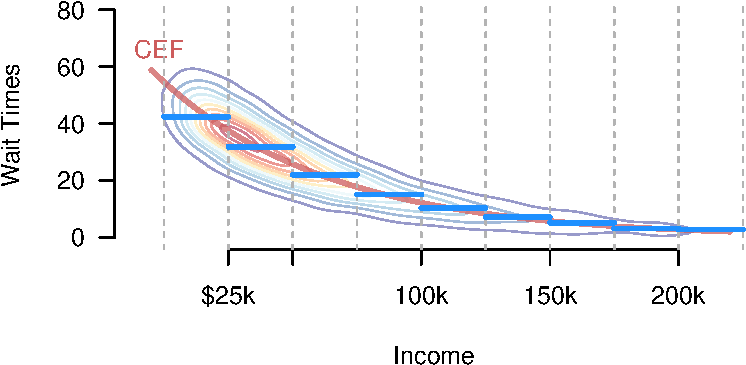
\includegraphics{./06_linear_model_files/figure-pdf/fig-cef-binned-1.pdf}

}

\caption{\label{fig-cef-binned}Hypothetical joint distribution of income
and poll wait times (contour plot), conditional expectation function
(red), and the conditional expectation of the binned income (blue).}

\end{figure}

Similarly, we could \textbf{assume} that the CEF follows a simple
functional form like a line, \[ 
\mu(x) = \E[Y_{i}\mid X_{i} = x] = \beta_{0} + \beta_{1} x.
\] This reduces our infinite number of unknowns (the conditional mean at
every possible income) to just two unknowns, the slope and intercept. As
we will see, we can use the standard ordinary least squares to estimate
these parameters. Notice again, though, that if the true CEF is
nonlinear this assumption is incorrect, any estimate based off this
assumption might be biased or even inconsistent.

We call the binning and linear assumptions on \(\mu(x)\)
\textbf{functional form} assumptions because restrict the class of
functions that \(\mu(x)\) can take. While powerful, these types of
assumptions can muddy the roles of defining the quantity of interest and
estimation. If our estimator \(\widehat{\mu}(x)\) performs poorly, it
will be difficult to tell if this is because the estimator is flawed in
some way or because our functional form assumptions are incorrect.

To help clarify these issues, we will pursue a different approach:
understanding what linear regression can estimate well under minimal
assumptions and then investigating how well this estimand approximates
the true CEF.

\hypertarget{population-linear-regression}{%
\section{Population linear
regression}\label{population-linear-regression}}

Let's set aside the idea of the conditional expectation function and
instead focus on finding the \textbf{linear} function of \(\X_i\) that
best predicts the outcome. Remember that a linear function can be
written \[ 
\bfx'\bfbeta = x_{1}\beta_{1} + x_{2}\beta_{2} + \cdots + X_{k}\beta_{k}.
\] We will define the \textbf{best linear predictor} (BLP) to be \[ 
\bbL[Y_{i} \mid \X_{i}] =\X_{i}'\bfbeta, \quad \text{where}\quad \bfbeta = \argmin_{\mb{b} \in \real^k}\; \E\bigl[ \bigl(Y_{i} - \mb{X}_{i}'\bfbeta \bigr)^2\bigr]
\] The BLP function \(\bbL[Y \mid \X]\) is the linear function of the
covariates that minimizes the mean squared prediction errors, where we
are averaging over the joint distribution of the data. If we have a
single covariate, this would be the population line of best fit. Again,
this function is a feature of the joint distribution of the data---the
DGP---and so represents something that we would like to learn about with
our sample. It is an alternative to the CEF for summarizing the
relationship between the outcome and the covariate, though we will see
that they will sometimes be equal to each other.

\begin{tcolorbox}[enhanced jigsaw, title=\textcolor{quarto-callout-note-color}{\faInfo}\hspace{0.5em}{Best linear projection assumptions}, breakable, titlerule=0mm, opacityback=0, rightrule=.15mm, bottomrule=.15mm, colframe=quarto-callout-note-color-frame, coltitle=black, colbacktitle=quarto-callout-note-color!10!white, bottomtitle=1mm, toptitle=1mm, colback=white, arc=.35mm, opacitybacktitle=0.6, toprule=.15mm, leftrule=.75mm, left=2mm]

Without some assumptions on the joint distribution of the data, The
following ``regularity conditions'' will ensure the existence of the
BLP:

\begin{enumerate}
\def\labelenumi{\arabic{enumi}.}
\tightlist
\item
  \(\E[Y^2] < \infty\) (outcome has finite mean/variance)
\item
  \(\E\Vert \mb{X} \Vert^2 < \infty\) (\(\mb{X}\) has finite
  means/variances/covariances)
\item
  \(\mb{Q}_{\mb{XX}} = \E[\mb{XX}']\) is positive definite (columns of
  \(\X\) are linearly independent)\\
\end{enumerate}

\end{tcolorbox}

Under these assumption, it is possible to derive a closed-form
expression for the \textbf{population coefficients} \(\bfbeta\) using
matrix calculus. To set up the optimization problem, we will find the
first order condition my taking the derivative of the expectation of the
squared errors. First, let's take derivative of the squared prediction
errors using the chain rule: \[ 
\begin{aligned}
  \frac{\partial}{\partial \mb{b}^{'}}\left(Y_{i} - \X_{i}'\mb{b}\right)^{2}
  &= 2\left(Y_{i} - \X_{i}'\mb{b}\right)\frac{\partial}{\partial \mb{b}'}(Y_{i} - \X_{i}'\mb{b})  \\
  &= -2\left(Y_{i} - \X_{i}'\mb{b}\right)\X_{i} \\
  &= -2\left(\X_{i}Y_{i} - \X_{i}\X_{i}'\mb{b}\right)
\end{aligned}
\] We can now plug this into the expectation to get the first-order
condition and solve for \(\bfbeta\), \[ 
\begin{aligned}
  0 &= -2\E[\X_{i}Y_{i} - \X_{i}\X_{i}'\bfbeta ]  \\
  \E[\X_{i}\X_{i}'] \bfbeta &= \E[\X_{i}Y_{i}],
\end{aligned}
\] which implies the population coefficients are \[ 
\bfbeta = \left(\E[\X_{i}\X_{i}']\right)^{-1}\E[\X_{i}Y_{i}] = \mb{Q}_{\mb{XX}}^{-1}\mb{Q}_{\mb{X}Y}
\] We now have an expression for the coefficients for the population
best linear predictor in terms of the joint distribution
\((Y_{i}, \X_{i})\). There are a couple facts that might be useful for
reasoning about this expression. Recall that
\(\mb{Q}_{\mb{XX}} = \E[\X_{i}\X_{i}']\) is a \(k\times k\) matrix and
\(\mb{Q}_{\X Y} = \E[\X_{i}Y_{i}]\) is a \(k\times 1\) column vector,
which implies that \(\bfbeta\) is also a \(k \times 1\) column vector.

\begin{tcolorbox}[enhanced jigsaw, title=\textcolor{quarto-callout-note-color}{\faInfo}\hspace{0.5em}{Note}, breakable, titlerule=0mm, opacityback=0, rightrule=.15mm, bottomrule=.15mm, colframe=quarto-callout-note-color-frame, coltitle=black, colbacktitle=quarto-callout-note-color!10!white, bottomtitle=1mm, toptitle=1mm, colback=white, arc=.35mm, opacitybacktitle=0.6, toprule=.15mm, leftrule=.75mm, left=2mm]

Intuitively, what is happening in the expression for the population
regression coefficients? It is helpful to separate out the intercept or
constant term so that we have \[ 
Y_{i} = \beta_{0} + \X'\bfbeta + e_{i},
\] so \(\bfbeta\) refers to just the coefficients on each of the
covariates. In this case, we can write the coefficients in more
interpretable way: \[ 
\bfbeta = \V[\X]^{-1}\text{Cov}(\X, Y), \qquad \beta_0 = \mu_Y - \mb{\mu}'_{\mb{X}}\bfbeta
\]

Thus, the population coefficients take the covariance between the
outcome and the covariates and ``divide'' it by information about
variances and covariances of the covariates. The intercept recenters the
regression so that projection errors are mean zero.

\end{tcolorbox}

With an expression for the population linear regression coefficients, we
can write the linear projection as \[ 
\bbL[Y_{i} \mid \X_{i}] = \X_{i}'\left(\E[\X_{i}\X_{i}']\right)^{-1}\E[\X_{i}Y_{i}] = \X_{i}'\mb{Q}_{\mb{XX}}^{-1}\mb{Q}_{\mb{X}Y}
\]

\hypertarget{projection-error}{%
\subsection{Projection error}\label{projection-error}}

The \textbf{projection error} is the difference between the actual value
of \(Y_i\) and the projection, \[ 
e_{i} = Y_{i} - \bbL[Y_{i} \mid \X_{i}] =  Y_i - \X_{i}'\bfbeta,
\] where it is hopefully clear that we have made no assumptions about
this error yet. It is simply the prediction error if we used the linear
projection to predict the outcome. Rewriting this definition, we can see
that we can always write the outcome as the linear projection plus the
projection error, \[ 
Y_{i} = \X_{i}'\bfbeta + e_{i}.
\] Notice that this looks suspiciously like we have made a linearity
assumption on the CEF or on the relationship between the outcome and the
covariates. But we haven't, we have just used the definition of the
projection error to write a statement that is tautological: \[ 
Y_{i} = \X_{i}'\bfbeta + e_{i} = \X_{i}'\bfbeta + Y_{i} - \X_{i}'\bfbeta = Y_{i}.
\] The key difference between this representation and the usual linear
model assumption is what properties \(e_{i}\) possesses.

One key property of the projection errors is that when the covariate
vector includes an ``intercept'' or constant term, the projection errors
are uncorrelated with the covariates. To see this, we first note that
\(\E[\X_{i}e_{i}] = 0\) since \[ 
\begin{aligned}
  \E[\X_{i}e_{i}] &= \E[\X_{{i}}(Y_{i} - \X_{i}'\bfbeta)] \\
                  &= \E[\X_{i}Y_{i}] - \E[\X_{i}\X_{i}']\bfbeta \\
                  &= \E[\X_{i}Y_{i}] - \E[\X_{i}\X_{i}']\left(\E[\X_{i}\X_{i}']\right)^{-1}\E[\X_{i}Y_{i}] \\
  &= \E[\X_{i}Y_{i}] - \E[\X_{i}Y_{i}] = 0
\end{aligned}
\] Thus, for every \(X_{ij}\) in \(\X_{i}\), we have
\(\E[X_{ij}e_{i}] =0\). If one of the entries in \(\X_i\) is a constant
1, then this also implies that \(\E[e_{i}] =0\). Together, these facts
imply that the projection error is uncorrelated with each \(X_{ij}\),
since \[ 
\cov(X_{ij}, e_{i}) = \E[X_{ij}e_{i}] - \E[X_{ij}]\E[e_{i}] = 0 - 0 = 0
\] Notice that we still have made no assumptions about these projection
errors except some mild regularity conditions on the joint distribution
of the outcome and covariates. Thus, in very general settings, we can
write the linear projection model \(Y_i = \X_i'\bfbeta + e_i\) where
\(\bfbeta = \left(\E[\X_{i}\X_{i}']\right)^{-1}\E[\X_{i}Y_{i}]\) and
conclude that \(\E[\X_{i}e_{i}] = 0\) by definition not by assumption.

The projection error is uncorrelated with the covariates, so does this
mean that the CEF is linear? Unfortunately, no because recall that while
independence implies uncorrelated, the reverse does not hold. So when we
look at the CEF, we have \[ 
\E[Y_{i} \mid \X_{i}] = \X_{i}'\bfbeta + \E[e_{i} \mid \X_{i}],
\] and the last term \(\E[e_{i} \mid \X_{i}]\) would only be 0 if the
errors were independent of the covariates so
\(\E[e_{i} \mid \X_{i}] = \E[e_{i}] = 0\). But nowhere in the linear
projection model did we assume this. So while we can (almost) always
write the outcome as \(Y_i = \X_i'\bfbeta + e_i\) and have those
projections error be uncorrelated with the covariates, it will require
additional assumptions to ensure that the true CEF is in fact linear
\(\E[Y_{i} \mid \X_{i}] = \X_{i}'\b\).

Let's take a step back. What have we shown here? In a nutshell, we have
shown that under very general conditions, a population linear regression
exists and we can write the coefficients of that population linear
regression as a function of expectations of the joint distribution of
the data. Why do we care about this? It turns out that the ordinary
least squares estimator, the workhorse regression estimator, targets
this quantity of interest in large samples, regardless of whether the
true CEF is linear or not. This means that even when a linear CEF
assumption is incorrect, OLS still targets a perfectly valid quantity of
interest: the coefficients from this population linear projection.

\hypertarget{linear-cefs-without-assumptions}{%
\section{Linear CEFs without
assumptions}\label{linear-cefs-without-assumptions}}

What is the relationship between the best linear predictor (which we
just saw exists very generally) and the CEF? To draw the connection,
remember a key property of the conditional expectation: it is the
function of \(\X_i\) that best predicts \(Y_{i}\). The population
regression was the best \textbf{linear} predictor, but the CEF is the
best predictor among all functions of \(\X_{i}\), linear or nonlinear,
that are nicely behaved. In particular, if we label \(L_2\) be the set
of all functions of the covariates \(g()\) such that they are finite
squared expectation, \(\E[g(\X_{i})^{2}] < \infty\), then we can show
that the CEF has the lowest squared prediction error in this class of
functions: \[ 
\mu(\X) = \E[Y_{i} \mid \X_{i}] = \argmin_{g(\X_i) \in L_2}\; \E\left[(Y_{i} - f(\X_{i}))^{2}\right],
\]

So we have established that the CEF is the best predictor and the
population linear regression \(\bbL[Y_{i}\mid \X_{i}]\) is the best
linear predictor. These two facts allow us to connect the CEF and the
population regression.

\leavevmode\vadjust pre{\hypertarget{thm-cef-blp}{}}%
\begin{theorem}[]\label{thm-cef-blp}

If \(\mu(\X_{i})\) is a linear function of \(\X_i\), then
\(\mu(\X_{i}) = \bbL[Y_{i}\mid \X_{i}] = \X_i'\bfbeta\).

\end{theorem}

This theorem says that if the true CEF is linear, then it is equal to
the population regression. The proof of this is straightforward: the CEF
is the best predictor, so if it is linear, it must also be the best
linear predictor.

In general, we are usually in the business of learning about the CEF so
we are unlikely to know if it truly is linear or not. In some
situations, however, we can show that the CEF is linear without any
additional assumptions. These will be situations when the covariates
take on a finite number of possible values. Suppose that we are
interested in the CEF of poll wait times for Black (\(X_i = 1\)) vs
non-Black (\(X_i = 0\)) voters. In this case, there are two possible
values of the CEF, \(\mu(1) = \E[Y_{i}\mid X_{i}= 1]\), the average wait
time for Black voters, and \(\mu(0) = \E[Y_{i}\mid X_{i} = 0]\), the
average wait time for non-Black voters. Notice that we can write the CEF
as \[ 
\mu(x) = x \mu(1) + (1 - x) \mu(0) = \mu(0) + x\left(\mu(1) - \mu(0)\right)= \beta_0 + x\beta_1,
\] which is clearly a linear function of \(x\). Based on this
derivation, we can see that the coefficients of this linear CEF have a
clear interpretation:

\begin{itemize}
\tightlist
\item
  \(\beta_0 = \mu(0)\): the expected wait time for a Black voter.
\item
  \(\beta_1 = \mu(1) - \mu(0)\): the difference in average wait times
  between Black and non-Black voters. Notice that it matters how
  \(X_{i}\) is defined here since the intercept will always be the
  average outcome when \(X_i = 0\) and the slope will always be the
  difference in means between the \(X_i = 1\) group and the \(X_i = 0\)
  group.
\end{itemize}

What about a categorical coviarate with more than two levels? For
instance, we might be interested in wait times by party identification,
where \(X_i = 1\) indicates Democratic voters, \(X_i = 2\) indicates
Republican voters, and \(X_i = 3\) indicates independent voters. How can
we possible write the CEF of wait times as a linear function of this
variable? That would assume that the difference between Democrats and
Republicans is the same as for Independents and Republicans. With more
than two levels, a categorical variable is better represented as a
vector of binary variables, \(\X_i = (X_{i1}, X_{i2})\), where \[ 
\begin{aligned}
  X_{{i1}} &= \begin{cases}
                1&\text{if Republican} \\
                   0 & \text{if not Republican}
              \end{cases} \\
X_{{i2}} &= \begin{cases}
                1&\text{if independent} \\
                   0 & \text{if not independent}
              \end{cases} \\
\end{aligned}
\] Clearly, these two indicator variables encode the same information as
the original three-level variable, \(X_{i}\). If I know the values of
\(X_{i1}\) and \(X_{i2}\), I know exactly what party to which \(i\)
belongs. Thus, the CEFs with repect to \(X_i\) and the pair of indicator
variables, \(\X_i\), is exactly the same, but the latter admits a very
nice linear representation, \[
\E[Y_i \mid X_{i1}, X_{i2}] = \beta_0 + \beta_1 X_{i1} + \beta_2 X_{i2},
\] where

\begin{itemize}
\tightlist
\item
  \(\beta_0 = \E[Y_{i} \mid X_{i1} = 0, X_{i2} = 0]\) is the average
  wait time for the group who does not get an indicator variable
  (Democrats in this case).
\item
  \(\beta_1 = \E[Y_{i} \mid X_{i1} = 1, X_{i2} = 0] - \E[Y_{i} \mid X_{i1} = 0, X_{i2} = 0]\)
  is the difference in means between Republican voters and Democratic
  voters, or the difference between the first indicator group and the
  baseline group.
\item
  \(\beta_2 = \E[Y_{i} \mid X_{i1} = 0, X_{i2} = 1] - \E[Y_{i} \mid X_{i1} = 0, X_{i2} = 0]\)
  is the difference in means between independent voters and Democratic
  voters, or the difference between the second indicator group and the
  baseline group.
\end{itemize}

This approach generalizes easily to categorical variables with an
arbitrary number of levels.

What have we shown? The CEF will be linear without additional
assumptions when there is a categorical covariate. We can show that this
continues to hold even when we have multiple categorical variables.
Suppose now that we have two binary covariates: \(X_{i1}=1\) indicating
a Black voter and \(X_{i2} = 1\) indicating an urban voter. With these
two binary variables, there are 4 possible values of the CEF: \[ 
\mu(x_1, x_2) = \begin{cases} 
 \mu_{00} & \text{if } x_1 = 0 \text{ and } x_2 = 0 \text{ (non-Black, rural)} \\
  \mu_{10} & \text{if }  x_1 = 1 \text{ and } x_2 = 0 \text{ (Black, rural)}\\
  \mu_{01} & \text{if }  x_1 = 0 \text{ and } x_2 = 1 \text{ (non-Black, urban)}\\
 \mu_{11} & \text{if }  x_1 = 1 \text{ and } x_2 = 1 \text{ (Black, urban)}
 \end{cases}
\] We can write this as \[ 
\mu(x_{1}, x_{2}) = (1 - x_{1})(1 - x_{2})\mu_{00} + x_{1}(1 -x_{2})\mu_{10} + (1-x_{1})x_{2}\mu_{01} + x_{1}x_{2}\mu_{11},
\] which we can rewrite as \[ 
\mu(x_1, x_2) = \beta_0 + x_1\beta_1 + x_2\beta_2 + x_1x_2\beta_3,
\] where

\begin{itemize}
\tightlist
\item
  \(\beta_0 = \mu_{00}\): average wait times for rural non-Black voters.
\item
  \(\beta_1 = \mu_{10} - \mu_{00}\): difference in means for rural Black
  vs rural non-Black voters..
\item
  \(\beta_2 = \mu_{01} - \mu_{00}\): difference in means for urban
  non-Black vs rural non-Black voters.
\item
  \(\beta_3 = (\mu_{11} - \mu_{01}) - (\mu_{10} - \mu_{00})\):
  difference in urban racial difference vs rural racial difference.
\end{itemize}

Thus, we can write the CEF with two binary covriataes as linear when the
linear specification includes and multiplicative interaction between
them (\(x_1x_2\)). This holds for all pairs of binary covariates and we
can generalize the interpretation of the coefficients in the CEF as

\begin{itemize}
\tightlist
\item
  \(\beta_0 = \mu_{00}\): average outcome when both variables are 0.
\item
  \(\beta_1 = \mu_{10} - \mu_{00}\): difference in average outcomes for
  the first covariate when second covariate is 0.
\item
  \(\beta_2 = \mu_{01} - \mu_{00}\): difference in average outcomes for
  the second covariate when the first covariate is 0.
\item
  \(\beta_3 = (\mu_{11} - \mu_{01}) - (\mu_{10} - \mu_{00})\): change in
  the ``effect'' of the first (second) covariate when the second (first)
  covariate goes from 0 to 1.
\end{itemize}

This result also generalizes to an arbitrary number of binary
covariates. If we have \(p\) binary covariates, then the CEF will be
linear with all two-way interactions, \(x_1x_2\), all three-way
interactions, \(x_1x_2x_3\), up to the \(p\)-way interaction
\(x_1\times\cdots\times x_p\). Furthermore, we can generalize to
arbitrary numbers of categorical variables by expanding each categorical
variable into a series of binary variables and then including all
interactions between the resulting binary variables.

We have established that when we have a set of categorical covariates,
the true CEF will be linear and we have seen the various ways to
represent that CEF. Notice that when we actually use, for example,
ordinary least squares, we are free to choose how to include our
variables. That means that we could run a regression of \(Y_i\) on
\(X_{i1}\) and \(X_{i2}\) without an interaction term. This model will
only be correct if \(\beta_3\) is actually equal to 0 and so the
interaction term is irrelevant. Because of this ability to choose our
models, it's helpful to have a language for models that capture the
linear CEF appropriately. We call a model \textbf{saturated} if there as
many coefficients as there are unique values of the CEF. A saturated
model by its nature can always be written as a linear function without
assumptions. The above examples show how to construct saturated models
in various situations.

\hypertarget{partitioned-regression}{%
\section{Partitioned regression}\label{partitioned-regression}}

When we have a regression with two groups of covariates,
\(\mb{V}_{i} = (\X_{i}, \mb{Z}_{i})\), we might want a formula for the
coefficients on just \(\X_i\). Given the matrix algebra involved in the
definition of the population regression coefficients, it isn't clear how
we might achieve this. It turns out we can obtain a formula for those
coefficients from a set of two population regressions.

In particular, let \(\bs{\delta}' = (\bfbeta', \bs{\gamma}')\) be the
coefficients the coefficients on the complete set of covariates, with
\(\bfbeta\) corresponding to \(\X_i\) and \(\bs{\gamma}\) corresponding
to \(\mb{Z}_i\). In other words, the linear projection in this case can
be written as \[ 
\bbL(Y_{i} \mid \mb{V}_{i})= \mb{V}_{i}'\mb{\delta} =  \X_{i}'\bfbeta + \mb{Z}_{i}'\bs{\gamma}.
\] To obtain an expression for \(\bfbeta\), we can first think of a
population regression of the covariates of interest \(\X_i\) on the
other covariates \(\mb{Z}_i\), \(\bbL(\X_{i} \mid \mb{Z}_{i})\). This
looks somewhat odd because we have a vector as the dependent variable,
but it represents the idea of running a separate regression of each
variable in \(\X_i\) on \(\mb{Z}_i\). So we end up with a matrix of
coefficients instead of a vector (one column for each variable in
\(\X_i\)), even though the expression for the linear projection does not
change much: \[ 
\bbL(\X_{i} \mid \mb{Z}_{i}) = \mb{Z}_{i}'\left(\E[\mb{Z}_{i}\mb{Z}_{i}']\right)^{{-1}} \E[\mb{Z}_{i}'\X_{i}].
\] These represent the best linear guess about the covariates of
interest given the other covariates. Let's define the prediction errors
\(\widetilde{\X}_i = \X_i - \bbL(\X_{i} \mid \mb{Z}_{i})\). Because
these are linear projection errors, we know from the above results that
they are uncorrelated with \(\mb{Z}_i\), which geometrically means they
are \textbf{orthogonal} to those covariates. Thus, we sometimes call the
transformation \(A - \bbL(A \mid B)\) \textbf{orthogonalizing} \(A\)
with respect to \(B\). The vector \(\widetilde{X}_i\) captures the
variation in \(\X_i\) that is not capture by a linear function of
\(\mb{Z}_i\). An amazing property of these errors is that when we
project \(Y_i\) onto just \(\widetilde{\X}_i\), we obtain the
coefficients on \(\X_i\) from the projection of \(Y_i\) on both \(\X_i\)
and \(\mb{Z}_i\): \[ 
\bfbeta = \left( \E[\widetilde{\X}_{i}\widetilde{\X}_{i}'] \right)^{-1}\E[\widetilde{\X}_{i}'Y_{i}].
\] The same result applies if we orthogonalize \(Y_i\) with respect to
\(\mb{Z}_i\) as well,\\
\[ 
\bfbeta = \left( \E[\widetilde{\X}_{i}\widetilde{\X}_{i}'] \right)^{-1}\E[\widetilde{\X}_{i}'\widetilde{Y}_{i}],
\] where \(\widetilde{Y}_i = Y_i - \bbL(Y_{i} \mid \mb{Z}_{i})\).

Why do care about this ability to partition the regression coefficients?
One reason is that it allows us to derive an interpretable expression
for each coefficient in the BLP. Let's change our partition slightly so
that \(\X_i = (X_{{ik}}, \X_{i,-k})\), where \(\X_{i,-k}\) is the vector
of covariates omitting the \(k\)th entry (we assume that \(\X_{i,-k}\)
includes the constant term 1). Based on the above, we can define
\(\widetilde{X}_{ik} = X_{ik} - \bbL(X_{ik}\mid \X_{i,-k})\) as the
\(k\)th variable othorgonalized with respect to rest of the variables.
Then the above partition results implies that \[ 
\beta_k = \frac{\cov(Y_i, \widetilde{X}_{ik})}{\V[\widetilde{X}_{ik}]}.
\] Thus, the population regression coefficient in the BLP is the
covariance of the outcome and the orthogonalized variable divided by the
variance of the orthogonalized value. More generally, this implies that
we could use a scatterplot of the outcome and the orthogonalized
covariate to explore the conditional relationship between these two
variable in a more flexible or exploratory manner.

\hypertarget{omitted-variable-bias}{%
\section{Omitted variable bias}\label{omitted-variable-bias}}

In many situations, we might need to choose to include a variable in a
regression or not, so it can be helpful to understand how this choice
might affect the population coefficients on the other variables in a the
regression. In particular, suppose we are considering whether to include
some variable \(Z_i\) in our regression where \(\X_i\) represents the
other covariates. Then we are deciding between the two projections \[ 
\bbL[Y_i \mid \X_i, Z_i] = \X_i'\bfbeta + Z_i\gamma, \qquad \bbL[Y \mid \X] = \X_i'\mb{\delta},
\] where we often refer to \(\bbL[Y_i \mid \X_i, Z_i]\) as the long
regression and \(\bbL[Y_i \mid \X_i]\) as the short regression.

Can we relate the coefficients on \(\X_i\) from these two regressions?
It turns out that we can using two property that linear projections
share with conditional expectations: the \textbf{law of iterated
projections}, \[
\bbL[Y_i \mid \X_i] = \bbL\left\{ \bbL[Y_i \mid \X_i, Z_i] \mid \X_i \right\},
\] and that linear projection is linear, so that
\(\bbL[A + B \mid C] = \bbL[A\mid C] + \bbL[B \mid C]\). Together, these
imply \[  
\begin{aligned}
 \bbL[Y_i \mid \X_i] &= \bbL[\X_i'\bfbeta + Z_i\gamma \mid \X_i] \\
 &= \bbL[\X_i\mid \X_i]'\bfbeta + \bbL[Z_i \mid \X_i]\gamma \\
 &= \X'_i\bfbeta + \bbL[Z_i \mid \X_i]\gamma
 \end{aligned}
\] We can write the regression/projection of \(Z_i\) on \(\X_i\) as
\(\bbL[Z_i \mid \X_i]= \X_i'\mb{\pi}\) and so \[ 
\bbL[Y_i \mid \X_i] = \X_i'(\bfbeta + \mb{\pi}\gamma), 
\] which implies that the short coefficients can be written as
\(\mb{\delta} = \bfbeta + \mb{\pi}\gamma\).

We can easily rewrite this to show that the difference between the
coefficients in these two projections is
\(\mb{\delta} - \bfbeta= \mb{\pi}\gamma\) or the product of the
coefficient on the ``excluded'' \(Z_i\) and the coefficient of the
included \(\X_i\) on the excluded. This difference is usually referred
to as the \textbf{omitted variable bias} of omitting \(Z_i\) under the
idea that \(\bfbeta\) is the true target of inference. But the result is
much broader than this since it just tells us how to relate the
coefficients of two nested projection.

\bookmarksetup{startatroot}

\hypertarget{least-squares}{%
\chapter{Least squares}\label{least-squares}}

In this chapter we explore the most widely used estimator for population
linear regressions: \textbf{ordinary least squares} (OLS). OLS is a
plug-in estimator for the best linear projection (or population linear
regression) described in the last chapter. Its popularity is due in part
to its easy of interpretation, its computational simplicity, and its
statistical efficiency.

Often, OLS is introduced along with an assumption of a linear model for
the conditional expectation. This chapter purposefully avoids this to
emphasize that OLS has a perfectly valid target of inference, the best
linear projection, regardless of the linearity of the conditional
expectation function.

\hypertarget{deriving-the-ols-estimator}{%
\section{Deriving the OLS estimator}\label{deriving-the-ols-estimator}}

\begin{tcolorbox}[enhanced jigsaw, title=\textcolor{quarto-callout-note-color}{\faInfo}\hspace{0.5em}{Assumption}, breakable, titlerule=0mm, opacityback=0, rightrule=.15mm, bottomrule=.15mm, colframe=quarto-callout-note-color-frame, coltitle=black, colbacktitle=quarto-callout-note-color!10!white, bottomtitle=1mm, toptitle=1mm, colback=white, arc=.35mm, opacitybacktitle=0.6, toprule=.15mm, leftrule=.75mm, left=2mm]

The variables
\(\{(Y_1, \X_1), \ldots, (Y_i,\X_i), \ldots, (Y_n, \X_n)\}\) are i.i.d.
draws from a common distribution \(F\).

\end{tcolorbox}

\hypertarget{bivariate-ols}{%
\section{Bivariate OLS}\label{bivariate-ols}}

\hypertarget{model-fit}{%
\section{Model fit}\label{model-fit}}

\hypertarget{matrix-form-of-ols}{%
\section{Matrix form of OLS}\label{matrix-form-of-ols}}

\hypertarget{projection}{%
\section{Projection}\label{projection}}

\hypertarget{outliers-leverage-points-and-influential-observations}{%
\section{Outliers, leverage points, and influential
observations}\label{outliers-leverage-points-and-influential-observations}}

\bookmarksetup{startatroot}

\hypertarget{references}{%
\chapter*{References}\label{references}}
\addcontentsline{toc}{chapter}{References}

\markboth{References}{References}

\hypertarget{refs}{}
\begin{CSLReferences}{0}{0}
\end{CSLReferences}



\end{document}
